\cotefile{58}
\scanpage{20}
\mspage{- 2 -}
\margin{n°358}

$V'_{(K)}$ dans $W$ et une seule telle que $\bar f'(v'\otimes 1)=f'(v')$ pour tout $v'$ dans $V'$.
Si $\lambda$ est un isomorphisme, l'application $K$-linéaire $\bar f'\mathbin{:}\lambda^{-1}$ est alors
l'unique application $K$-linéaire de $V$ dans $W$ prolongeant $f'$ ; autrement dit,
a) implique b). D'autre part, si b) est satisfaite, il existe une application $K$-linéaire $\mu$ de $V$ dans $V'_{(K)}$ telle que $\mu(v')=v'\otimes 1$ pour tout $v'$
dans $V'$ ; il est immédiat que $\lambda$ et $\mu$ sont des applications réciproques, et
par suite $\lambda$ est une bijection. On a donc prouvé que a) équivaut à b).

Par ailleurs, pour toute base $B'$ de $V'$ sur $K'$, l'ensemble $B$ des éléments
$v'\otimes 1$ de $V'_{(K)}$ (pour $v'$ parcourant $B'$) est une base de $V'_{\inserted{(K)}}$ sur $K$, et $\lambda$
transforme $B$ en $B'$. Pour que l'application $K$-linéaire $\lambda$ soit bijective, il
faut que l'image par $\lambda$ de toute base de $V'_{(K)}$ soit une base de $V$ sur $K$, et
il suffit qu'il en soit ainsi pour une seule base. Ceci prouve l'équivalence
de a), c) et d).

Comme toute partie de $V'$ libre sur $K'$ est contenue dans une base de $V'$
sur $K'$, c) implique e). Enfin, supposons e) satisfaite ; si $B'$ est une base
de $V'$ sur $K'$, c'est une partie de $V$ libre sur $K$, et comme $B'$ engendre $V'$
sur $K'$, donc $V$ sur $K$ d'après e), on voit que $B'$ est une base de $V$ sur $K$ ;
on a donc prouvé que e) implique c). C.Q.F.D.

DEFINITION 1.- \uline{Soient} $V$ \uline{un espace vectoriel à droite sur un corps} $K$ \uline{et} $K'$ \uline{un}
\uline{sous-corps de} $K$. \uline{On appelle} $K'$-\uline{structure sur} $V$ \uline{tout sous-espace} $K'$-\uline{vectoriel}
$V'$ \uline{de} $V$ \uline{qui vérifie les conditions équivalentes de la prop.1}. \uline{On dit que les}
\uline{éléments de} $V'$ \uline{sont les vecteurs rationnels sur} $K'$.

2. \uline{Rationalité pour un sous-espace.}

DEFINITION 2.- \uline{Soient} $V$ \uline{un espace vectoriel à droite sur le corps} $K$ \uline{et} $V'$
\uline{une} $K'$-\uline{structure sur} $V$. \uline{On dit qu'un sous-espace} $K$-\uline{vectoriel} $W$ \uline{de} $V$ \uline{est}
\uline{rationnel sur} $K'$ \uline{s'il est engendré sur} $K$ \uline{par} $W\cap V'$.

\margin{19}
\scanpage{21}

\uline{Lemme 4} Soit $X$ un \unsure{préschéma}
noethérien connexe, \inserted{dont les composantes irréductibles de dim $\geq h$, et}
tel que pour tt pt \uline{fermé} $x\in X$, $(\operatorname{Spec}\underline{O}_{X,x})'$ soit connexe
en dim $\geq\unsure{k|h}\deleted{\unsure{au}}$. Alors $X$ est connexe
en dim $\geq h$.

\margin{\uline{Peut se renforcer :} pour tt $x$ tel que $\dim\bar x<h$,
$(\operatorname{Spec}\underline{O}_{X,x})'$ connexe.
Mais il suffit de renvoyer au \unsure{lemme} \unsure{bien} \unsure{général}
dans EGA \uline{IV} § de \unsure{conn. géom.}, dernier N°.
}

\deleted{\unsure{Supposons}}\inserted{Soit} en effet \deleted{\unsure{un}} $Z$ un
fermé de $X$ de dim $<h$,
prouvons que $Z$ ne déconnecte pas $X$.
\deleted{\unsure{On le suppose}} S'il le déconnectait,
Alors on aurait
\[
U=X-Z=U'\cup U'',
\]
avec $U'$, $U''$ fermés de $U$, $U'\cap U''=\varnothing$,
Soit $X'=\bar U'$, $X''=\bar U''$, donc \inserted{car $U$ dense}
\deleted{$X=(Z\cup X')\cup X''$, \deleted{\unsure{donc}} donc $(Z\cup X')\cap X''\ne\varnothing$}
dans $X$, $\unsure{X|X^2}=X'\cup X''$, donc $X'\cap X''\ne\varnothing$.
Soit $z$ un pt fermé de $X'\cap X''$.
Alors \unsure{s'induisant} sur $\operatorname{Spec}\underline{O}_{X,z}=X_z$,
on voit que $Z_z$ déconnecte $X_z$,
ou $Z'_z$ déconnecte $X'_z$, \unsure{d'où une}

\margin{20}
\scanpage{22}
\mspage{- 3 -}
\margin{n°355}

Le $B$-module $E\otimes_A F$ est réunion des sous-modules $E'\otimes_A F$, $E'$ parcourant
l'ensemble des sous-modules de type fini de $E$. Si donc $\underline P$ appartient à
$\operatorname{Ass}_B(E\otimes_A F)$, il existe un $E'$ de type fini tel que $\underline P\in\operatorname{Ass}_B(E'\otimes_A F)$. D'après
(ii), il existe $\underline p\in\operatorname{Ass}_A(E')$ tel que $\underline P\in\operatorname{Ass}_B(F/\underline pF)$ ; comme
$\operatorname{Ass}_A(E')\subset\operatorname{Ass}_A(E)$, cela achève de démontrer la proposition.

COROLLAIRE.- \uline{Si} $A$ \uline{est noethérien}, \uline{et si} $\underline P\in\operatorname{Ass}_B(E\otimes_A F)$, \uline{on a}
$\pi^{-1}(\underline P)\in\operatorname{Ass}_A(E)$.

Cela résulte des propositions 1 et 2.

\uline{Remarques}.-

1) Supposons $A$ \uline{et} $B$ \uline{noethériens}. Soit $\underline P$ un idéal premier de $B$, et soit
$\underline p=\pi^{-1}(\underline P)$. Soit $S=A-\underline p$, et soit $k(\underline p)=S^{-1}(A/\underline p)$ le corps des fractions
de $A/\underline p$. Puisque $\underline P$ contient $\pi(\underline p)$, il définit un idéal premier de $B/\underline pB$, et
puisqu'il ne rencontre pas $S$, il définit aussi un idéal premier, noté $\underline{P'}$,
de $S^{-1}(B/\underline pB)=k(\underline p)\otimes_A B$. Alors, \uline{pour que} $\underline P\in\operatorname{Ass}_B(E\otimes_A F)$, \uline{il faut et il}
\uline{suffit que} $\underline p\in\operatorname{Ass}_A(E)$ \uline{et} $\underline{P'}\in\operatorname{Ass}_{k(\underline p)\otimes_A B}(k(\underline p)\otimes_A F)$.

Vu la prop.2, tout revient à voir que les conditions
\[
\text{`` }\underline P\in\operatorname{Ass}_B(F/\underline pF)\text{ ''}\quad\text{et}\quad
\text{`` }\underline{P'}\in\operatorname{Ass}_{k(\underline p)\otimes_A B}(k(\underline p)\otimes_A F)\text{ ''}
\]
sont équivalentes, ce qui résulte de la prop.5 du §1 (c'est ici que l'on
utilise l'hypothèse noethérienne sur $B$).

[D'après Grothendieck, l'énoncé ci-dessus est celui que l'on utilise dans
les schémas (le produit tensoriel par $k(\underline p)$ s'interprétant comme le passage
à la ``fibre au-dessus de $\underline p$ '').]

2) La proposition 2 s'applique notamment lorsque $B$ \uline{est plat sur} $A$ et que
l'on prend $F=B$. Le module $E\otimes_A F$ est alors simplement le module $E_{(B)}$
\uline{déduit de} $E$ \uline{par extension des scalaires}.

On recopie ensuite les deux dernières pages de l'Etat 1.

\begin{center}-:-:-:-\end{center}
\margin{21}
\scanpage{23}

\uline{Théorème 2} Soit $f:X\longrightarrow Y$ un
morphisme \deleted{\unsure{loc. de t.f.}} propre de
préschémas \inserted{\unsure{loc}} \unsure{noeths}, avec $Y$ intègre,
$y_0\in Y$, $y_1$ \deleted{\unsure{une générisation}}
\deleted{le \unsure{pt gén. de $Y$}}\inserted{le pt gén de $Y$}.
On suppose
\deleted{que l'on est dans le \unsure{cas des} \unsure{variétés}}
\deleted{\unsure{intég}}
\margin{\figure{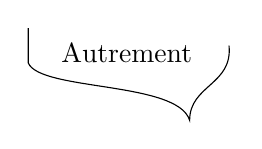
\begin{tikzpicture}[x=1cm,y=1cm]
\node at (0,0) {\deleted{\unsure{Autrement}}};
\draw (-1.25,.32) -- (-1.25,-.12) .. controls (-1.1,-.48) and (.65,-.35) .. (.8,-.85)
.. controls (.8,-.4) and (1.35,-.4) .. (1.3,.1);
\end{tikzpicture}}}

\margin{?}
\deleted{(a)} (a) $Y$ est [\unsure{géom.}$^{\unsure{t}}$] unibranche en $y_0$,
et les composantes irréductibles de
$X$ dominent $Y$.

\inserted{(b) les composantes irréductibles de}
\deleted{(b) $f$ est \unsure{universellement ouvert}.}
\deleted{\unsure{$f$}} \uline{$X_1$ sont} de dim $\geq\unsure{h+1|h_0}$, et $X_1$ est
connexe en dim $\geq h$.

Alors (les composantes irréductibles
de $X_0$ sont de dim $\geq h+1$) et
$X_0$ est \uline{connexe} en dim $\geq h$.

L'assertion \unsure{entre} parenthèses est
bien connue par le \unsure{théorème} des 2
dimensions, et n'utilise pas l'hypothèse
unibranche. Celle-ci sert uniquement
à appliquer le \uline{th. de \unsure{connexion|connexité}},
qui assure que $X_0$ est connexe.

\margin{22}
\scanpage{24}
\mspage{- 2 -}
\margin{n°355}

d'où $\operatorname{Ass}_B(F/\underline pF)\subset\operatorname{Ass}_B(E\otimes_A F)$, ce qui démontre l'inclusion $(\ast)$.

On va maintenant supposer que $A$ est \uline{noethérien}, et démontrer l'inclusion
opposée. On procèdera par étapes :

(i) $E$ \uline{est un module de type fini et} $\operatorname{Ass}_A(E)$ \uline{est réduit à un élément} $\underline p$.

D'après le th. 1 du §1, il existe une suite de composition $(E_i)_{0\leq i\leq n}$ de
$E$ telle que $E_i/E_{i+1}$ soit isomorphe à $A/\underline p_i$, où $\underline p_i$ est un idéal premier de $A$.
D'après le th.2 du §1, tous les $\underline p_i$ contiennent $\underline p$. Du fait que $F$ est $A$-plat,
les $E_i\otimes_A F$ forment une suite de composition de $E\otimes_A F$, et
$(E_i\otimes_A F)/(E_{i+1}\otimes_A F)$ s'identifie à $A/\underline p_i\otimes_A F=F/\underline p_iF$. En appliquant la
prop.3, on en déduit :
\[
\operatorname{Ass}_B(E\otimes_A F)\subset\bigcup\operatorname{Ass}_B(F/\underline p_iF).
\]

Soit donc $\underline P\in\operatorname{Ass}_B(E\otimes_A F)\cap\operatorname{Ass}_B(F/\underline p_iF)$. Si $\underline p_i\ne\underline p$, il existe $a\in\underline p_i$,
$a\notin\underline p$. D'après le cor.2 à la prop.2 du §1, l'homothétie de
rapport $a$ est injective dans $E$, donc celle de rapport $\pi(a)$ est injective
dans $E\otimes_A F$ ; mais d'autre part, $\pi(a)$ annule $F/\underline p_iF$, d'où $\pi(a)\in\underline P$, contradiction.
Ainsi $\underline p_i$ est nécessairement égal à $\underline p$, ce qui démontre la proposition dans le cas considéré.

(ii) $E$ \uline{est un module de type fini}.

Soient $\underline p_i$ les éléments de $\operatorname{Ass}_A(E)$, et soit $0=\bigcap Q_i$ une décomposition
primaire réduite correspondante (cf. §2, n°2). Le module $E$ se plonge dans
la somme directe des $E_i=E/Q_i$, et $E\otimes_A F$ se plonge dans la somme directe
des $E_i\otimes_A F$. On en déduit :
\[
\operatorname{Ass}_B(E\otimes_A F)\subset\bigcup\operatorname{Ass}_B(E_i\otimes_A F).
\]
D'après (i), on a $\operatorname{Ass}_B(E_i\otimes_A F)=\operatorname{Ass}_B(F/\underline p_iF)$, d'où la proposition dans
ce cas.

(iii) \uline{Cas général}.

\margin{23}
\scanpage{25}

Le Lemme 4 nous ramène
alors à vérifier le

\uline{Lemme 5} (\unsure{notations} comme le th).

Sous les conditions du th, mais
sans \deleted{\unsure{supposer} \illegible{3}}
\inserted{supposer $\unsure{y_0|Y}$ \deleted{\unsure{géom.}} \uline{unibranche}}
en $y_0$, \inserted{ni $f$ propre,} pour tt pt fermé \inserted{$x$} de $X_0$,
\deleted{l'anneau local} $\operatorname{Spec}(\unsure{\widehat{\underline O}|\underline O}_{X_0,x})$ est
connexe en dim $\geq h$

\margin{\unsure{Bien plutôt} : tout $x$ tel que $\dim\bar x<h$,
$(\operatorname{Spec}\underline{O}_{X_0,x})'$ est connexe}

En effet, le lemme 1 \inserted{\figure{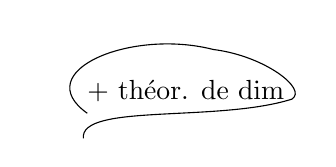
\begin{tikzpicture}[x=1cm,y=1cm]
\node at (0,0) {+ \unsure{théor. de dim}};
\draw (-1.25,-.28) .. controls (-2,.25) and (-.7,.8) .. (.35,.53)
.. controls (1,.45) and (1.55,.03) .. (1.35,-.1)
.. controls (.4,-.4) and (-1.35,-.15) .. (-1.3,-.6);
\end{tikzpicture}}} nous
ramène facilement, utilisant
l'hypothèse sur $X_1$, au cas où
$X_0$ est \uline{irréductible} \deleted{de dim $\geq h+1$},
donc $X$ \uline{irréductible} dominant $Y$,
\inserted{donc $=$ intègre comme $Y$.}
On peut supposer par une réduction
facile (?) au cas où
\deleted{``le \unsure{complété de} \illegible{2}}
\inserted{$\underline{O}_{Y,y_0}$ est}
\inserted{\unsure{formellt} équidimensionnel}
\deleted{\unsure{dimensions} \illegible{2} pour $\underline{O}_{Y,y_0}$''.}
\margin{conjecture}

D'où
\[
\dim\underline{O}_{X,x}
=\underbrace{\dim\underline{O}_{Y,y_0}}_{n}
+\underbrace{\dim X_1}_{\geq h+1}
\]

\margin{24}
\scanpage{26}

\begin{center}
ALGEBRE COMMUTATIVE

CHAPITRE IV - DECOMPOSITION PRIMAIRE

\uline{Décomposition primaire et extension des scalaires} (Etat 2)

-:-:-
\end{center}
\margin{Rédaction n°355}

L'état 1 porte le n°352. Après l'avoir lu (et même avant), Grothendieck
a signalé au rédacteur qu'on pouvait généraliser le résultat principal, en
remplaçant l'un des anneaux par un module. La démonstration s'étend sans
changement, et c'est bien plus joli. Le rédacteur en a profité pour enlever
quelques hypothèses noethériennes inutiles.

\begin{center}-:-:-\end{center}

Dans tout ce qui suit, on désigne par $A$ et $B$ deux anneaux commutatifs,
et l'on considère un homomorphisme $\pi:A\longrightarrow B$. Cet homomorphisme fait de
$B$ une $A$-algèbre. On se donne en outre un $B$-module $F$ que l'on suppose \uline{plat}
\uline{sur} $A$.

PROPOSITION 1.- \uline{Soit} $\underline p$ \uline{un idéal premier de} $A$. \uline{Pour tout} $\underline P\in\operatorname{Ass}_B(F/\underline pF)$ \uline{on a}
$\pi^{-1}(\underline P)=\underline p$.

Puisque $\pi(\underline p)$ annule $F/\underline pF$, on a $\pi(\underline p)\subset\underline P$, d'où $\underline p\subset\pi^{-1}(\underline P)$. D'autre
part, si $a\in A-\underline p$, l'homothétie de rapport $a$ est injective dans $A/\underline p$, donc
aussi (puisque $F$ est $A$-plat) dans $F/\underline pF$, ce qui montre que $\pi(a)\notin\underline P$, CQFD.

PROPOSITION 2.- \uline{Soit} $E$ \uline{un} $A$-\uline{module}. \uline{On a} :
\[
(\ast)\qquad
\operatorname{Ass}_B(E\otimes_A F)\supset\bigcup_{\underline p\in\operatorname{Ass}_A(E)}\operatorname{Ass}_B(F/\underline pF)
\]
\uline{Lorsque} $A$ \uline{est noethérien}, \uline{l'inclusion} $(\ast)$ \uline{est une égalité}.

Soit $\underline p\in\operatorname{Ass}_A(E)$. Par définition de $\operatorname{Ass}_A(E)$, il existe une suite exacte :
\diagram{\begin{tikzcd}
0\arrow[r]&A/\underline p\arrow[r]&E.
\end{tikzcd}}

Puisque $F$ est plat sur $A$, on en déduit une suite exacte :
\diagram{\begin{tikzcd}
0\arrow[r]&F/\underline pF\arrow[r]&E\otimes_A F,
\end{tikzcd}}

\margin{25}
\scanpage{27}

Donc divisant $O_{X,x}$ par un idéal défini
par $\unsure{n|h}$ \unsure{élts}, on \deleted{\unsure{démontre}} trouve par
le th général \deleted{\unsure{sur}} (\unsure{puisque} :
$\underline O_{X,x}$ intègre \unsure{formellt} \unsure{équidim.} de
dim $\geq K+1=(n+h)+1$ ] un anneau
qui est connexe en dim $\geq\deleted{\unsure{(n+h)}}\inserted{K-n}$
$=\unsure{k|h}$, cqfd.

\uline{Cor. 1} au th. 2 Variante
avec \deleted{\unsure{connexité}} ``géométriquement \deleted{\unsure{int}}
unibranche'', $*$ et fibres géométriques.

\uline{Cor. 2} Variante avec $f$ propre
\unsure{mais|univ.} ouvert.

\uline{Cor. 3} $X\subset P^n_k$, \deleted{$X$ \unsure{de dim}}
\inserted{les composantes}
de $X$ de dim $\geq h+1$, et $X$ connexe
en dim $\geq h$. Alors pour $H$ système
de $\ell$ hyperplans $H_1$--$H_\ell$, \inserted{de même,} \deleted{\unsure{et}}
$X\cap H_1\cap\cdots\cap H_\ell=Y$
\unsure{satisfait les} conditions analogues avec
$h-\ell$ au lieu de $h$.

\margin{Généralisation au cas d'un morphisme
$X\longrightarrow P^n_k$.
Peut-on généraliser de façon analogue
le th. local ? Facile, \unsure{en}
utilisant le \unsure{th.} \unsure{EGA},
\unsure{connexité} \unsure{initial}.
}

\margin{26}
\scanpage{28}

\begin{flushright}
\deleted{\unsure{Théorie}.}\inserted{\uline{Couples de}}
\uline{Lefschetz-Grauert}

$(X,Y)$
\end{flushright}

\margin{27}
\scanpage{30}

\uline{\mspage{\uline{III} \unsure{0}}}

\uline{Introduction}

Dans le par. \unsure{4}, nous avons vu \deleted{que} lorsque
$X$ est propre sur $Y$ \deleted{loc. noeth, \unsure{I-adique}
\unsure{complet}, \inserted{\unsure{pour} $A$}}
\deleted{et si on \unsure{avait}} et si $Y'$ est une partie
fermée de $Y$, $X'=f^{-1}(Y')$, la \inserted{en particulier,}
commutation des foncteurs \deleted{$R^if$ et $R^i\hat f$ aux}
``images directes supérieures'' aux foncteurs complétion
[le long de $Y'$, resp $X'$].
Lorsque $Y$ était le spectre d'un anneau \deleted{\unsure{local}}
noeth $I$-adique complet, et $Y'=V(\unsure{I})$, ces résultats,
complétés par un th. d'existence (par 5), s'expriment
\deleted{en disant} \inserted{\unsure{en termes}}
\deleted{que $F'\unsure{\mathbin{-}|\longrightarrow}F'_{Y'}$ est un}
par l'équivalence de la catégorie des \deleted{faisceaux}
\inserted{Modules} coh. sur $\unsure{X'|X}$ et de la catégorie
des \unsure{pro-Modules} coh. sur $\unsure{X'_{Y'}|\widehat X_{Y'}}$,
\uline{compatible} avec les foncteurs des modules de cohomologie.

Dans ce par., nous \deleted{\unsure{généraliserons}}
\inserted{\unsure{voulons|montrons}}, que ces résultats \unsure{puissent}
se généraliser à certaines situations, où $f:X'\longrightarrow X$
n'est plus supposé propre [p. ex. $f$ une imm. ouverte\ldots];
la \inserted{seule} \unsure{différence} \unsure{essentielle}
est que \unsure{ici} \unsure{on se borne}
\deleted{\unsure{en ce qui concerne} des \unsure{énoncés}
à préciser \unsure{les} \unsure{th.} \unsure{de}
\unsure{connexité} et leurs \illegible{2}}
\inserted{\unsure{des bornes} \unsure{cohom.} qui
\unsure{pour des raisons} \unsure{seront}
$\unsure{\leq n}$, par \unsure{récurrence}.}
\unsure{du} \unsure{théor.} (cf N° 2).
La méthode sera celle des par 4 et 5,
\inserted{\unsure{d'ailleurs très générale}}
en utilisant des \uline{th. de finitude}
\inserted{(N° 1)} \deleted{\unsure{pour} les \unsure{cohomologies}
$\unsure{f_*}$ \unsure{qui se trouvent}}
\unsure{convenables}, faisant intervenir des propriétés
\deleted{\unsure{cohomologiques} \unsure{supposées}}
\inserted{s'expriment :}
locales des faisceaux envisagés, qui s'expriment :

\margin{29}
\scanpage{31}

l'aide de la notion de \uline{profondeur}.

Les résultats \inserted{ainsi} obtenus sont l'outil technique
principal pour un \deleted{\unsure{développ.}}
\inserted{développement} systématique de
\deleted{propriétés} \inserted{certains théorèmes}
du type de ``Lefschetz'', comparant les propriétés géométriques
d'un schéma $X$ à celles de certains \inserted{sous-schémas}
diviseurs $Y$, \deleted{(section hyperplane)}
\deleted{\unsure{de} $X$} \inserted{\unsure{sur} $X$},
\uline{via} les propriétés du complété formel $X_{/Y}$, \unsure{etc}.
\deleted{Ils \unsure{présentent} \unsure{un} \illegible{2}
\unsure{l'observation} \unsure{faite} \unsure{plus} \unsure{explicite}.}
Ils sont applicables par exemple
\inserted{(après des \unsure{procédés usuels} de passage aux
\unsure{cônes projetants})}
au cas d'une variété projective $X$ et une section hyperplane
convenable, moyennant des hypothèses \deleted{de \unsure{rang}}
convenables sur la profondeur de $X$.
\deleted{\unsure{Ces} \unsure{résultats}}

\inserted{Dans ce cas}
\deleted{\unsure{nous aurons donc} à préciser.}
\uline{Le théorème} \deleted{\unsure{est dû}}
par H. Grauert qui avait d'ailleurs
\deleted{\unsure{été} \unsure{démontré} par \unsure{nous}}
(\deleted{\unsure{Bourbaki}} dès 1958,
(utilisant les th. de \unsure{nullité} de Serre [\ ]) [\ ])
\deleted{\unsure{et montrant que dans la situation précédente}}
\deleted{\unsure{il} \unsure{était} \illegible{2}}

(i) \inserted{Pour tt $F$ loc. libre,}
\[
H^i(X,F)\longrightarrow H^i(\hat X,\hat F)
\quad\text{est bijectif}
\]
pour des \deleted{petits} $i\leq n$
\deleted{[$n$ \unsure{dépendant de}]}
\inserted{$\unsure{\leq}\operatorname{prof}F-2$}.

(ii) si un faisceau formel loc. libre
$\unsure{\mathfrak F|\mathcal F}$ sur $X_{/Y}$,
\deleted{$\unsure{\hat{\mathfrak F}}$ \unsure{est}}
\inserted{et si $\operatorname{prof}(\unsure{O_{X}})\geq2$,}
alors pour $n$ \deleted{\unsure{corps de sections}}
grand, $\unsure{\mathfrak F|\mathcal F}(n)$ est engendré
par ses sections [\unsure{et}] sur un ens. fini --
\deleted{[et \unsure{pour les sections}, \unsure{voir}
\unsure{N°} \unsure{d'un} \unsure{Grothendieck},
\unsure{cela} \unsure{est} \unsure{utile}]}
comme nous montrerons],
(\unsure{Cela qui} implique \inserted{p. ex.}
déjà ce th de Lefschetz pour le groupe fondamental annoncé dans [\ ]).
$\unsure{\rho|p}$

\margin{$\unsure{\rho|p}$ La théorie développée ici et
\unsure{plus loin} en précisera et en généralisera les résultats
de Grauert.}

\margin{30}
\scanpage{32}

\figure{\begin{tikzpicture}[x=1cm,y=1cm,every node/.style={anchor=north west,align=left}]
\draw (0.35,0.15)--(0,0.15)--(0,-12.55) to[out=-90,in=180] (0.3,-12.8);
\draw (0,-11.15)--(0.4,-11.15);
\node[text width=13.6cm] at (0.4,0) {1. Généralisation des th. de finitude formelle, et du th. de comparaison. Application : un th. d'existence};
\node[text width=13.6cm] at (0.4,-1.35) {2. Le Théorème de finitude locale et ses applications.};
\node[text width=13.6cm] at (0.4,-2) {\deleted{3. Fermés de Lefschetz-Grauert; Remarques.}};
\node[text width=13.6cm] at (0.4,-2.9) {\deleted{4. \unsure{Premières} propriétés des \uline{Exemples} \unsure{fondamentaux}}};
\node at (10.5,-2.65) {\inserted{1}};
\draw[rounded corners] (0.35,-1.98) rectangle (12.4,-3.42);
\draw (0.45,-3.3)--(1.25,-2.1)--(1.9,-3.35)--(2.55,-2.1)--(3.35,-3.35)--(4,-2.1)--(4.7,-3.35)--(5.4,-2.1)--(6.3,-3.35)--(7,-2.1)--(7.9,-3.35)--(8.7,-2.1)--(9.5,-3.35)--(10.3,-2.1)--(11.1,-3.35)--(12.1,-2.2);
\node[text width=13.6cm] at (0.65,-3.85) {3. Cas particulier \unsure{I|II} : \deleted{Étude}\inserted{\unsure{théorie}} dans \deleted{\unsure{les}} schémas locaux.};
\node[text width=13.6cm] at (0.65,-4.85) {4. Cas particulier 2 : \deleted{Étude}\inserted{\unsure{théorie}} des schémas projectifs \inserted{\unsure{quelconques|réguliers}}};
\node[text width=13.6cm] at (0.65,-6.15) {5. Fermés de Lefschetz-Grauert. Remarques, exemples.};
\node at (0.65,-7.2) {6. Propriétés liées aux $\pi_0,$};
\node (pi) at (7.1,-7.2) {$\pi_1$};
\node at (7.7,-7.2) {, Pic.};
\draw (7.45,-7.48) ellipse[x radius=.32,y radius=.5];
\node at (0.35,-8.25) {[7. Propriétés de permanence]};
\node (eight) at (0.65,-9.5) {8.};
\draw (0.9,-9.7) ellipse[x radius=.46,y radius=.55];
\node[text width=12cm] at (1.65,-9.45) {Théorèmes de pureté, et Théorèmes de Lefschetz pour le $\pi_1$.};
\node[draw,rounded corners,rotate=28,text width=3.1cm] (m) at (-2,-6.65) {\margin{\unsure{utilise|utiliser} IV, \S\ sur les morphismes étales\ldots}};
\draw[->] (m.south east) to[out=12,in=175] (7.25,-6.95);
\draw[->] (-.95,-7.9) to[out=-55,in=150] (0.45,-9.45);
\node at (0.7,-11.45) {\deleted{\unsure{9}}};
\draw (1,-11.8) ellipse[x radius=.45,y radius=.5];
\draw (0.65,-11.45)--(1.3,-11.8)--(0.65,-12)--(1.25,-11.5)--(.75,-12.15)--(1.3,-11.65);
\node at (0.7,-12.35) {9};
\node[text width=12cm] at (2,-12) {\uline{Anneaux} \deleted{\illegible{1}} \uline{quasi-factoriels} et \uline{th de} \\ \uline{Lefschetz pour Pic.}};
\end{tikzpicture}}

\margin{31}
\scanpage{33}

\uline{Fermés de Lefschetz-Grauert}

1) Définitions, remarques

\uline{Déf} Soit $X$ un préschéma loc noeth, $Y$ une partie
fermée, $n$ un entier. On dit que $Y$ a la propriété
$(LG)_n$ dans $X$ \deleted{\unsure{propriété} \unsure{d'ordre} $n$},
si pour \unsure{tt|$\forall$} $F$ loc. libre sur $X$,
\[
(\alpha)\qquad H^i(X,F)\longrightarrow H^i(X_{/Y},F_{/Y})
\deleted{\unsure{\text{est}}}
\]
est bijectif pour $i\leq n$, \inserted{et injectif pour $i=n+1$.}

\margin{Inutile}

On dit que $Y$ a la propriété $LG$ \inserted{faible en $X$} si
\inserted{pour tout $F$ loc. libre sur $X$,}
\deleted{elle a la propriété $(LG)_0$}
\[
H^0(X,F)\xrightarrow{\sim}H^0(X_{/Y},F_{/Y})
\]
[i.e. $F\longmapsto F_{/Y}$ est pl. fid. des Mod. loc. libres
sur $X$ \unsure{dans ceux} sur $X_{/Y}$]

On dit que $Y$ a la propriété $LG$ \deleted{dans $X$} si
$\forall$ voisinage ouvert $U$ de $Y$, \deleted{$Y$}
\inserted{\unsure{la dite} propriété $LG$ faible en $U$.}
\deleted{\unsure{si}} $Y$ a la propriété $LG$,
\inserted{\deleted{\unsure{définie}} si elle a la propriété $LG$,}
et si de plus \deleted{pour}
$\forall$ $\unsure{\mathfrak F|\mathcal F}$ loc. libre sur $X_{/Y}$,
\deleted{\unsure{il}} est isom. à un faisceau de la forme
$F_{/Y}$, avec $F$ loc libre sur un voisinage ouvert $U$ de $Y$.

\margin{\figure{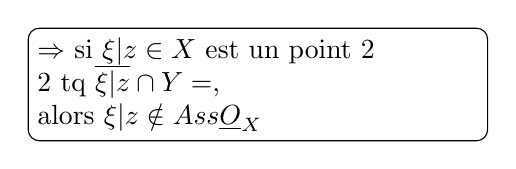
\begin{tikzpicture}
\node[draw,rounded corners,align=left,text width=5.6cm] {$\Rightarrow$ si $\unsure{\xi|z}\in X$ est un
\deleted{\unsure{point} \illegible{2}}\newline
\deleted{\illegible{2}}
\unsure{tq} $\overline{\unsure{\xi|z}}\cap Y=\varnothing$,\newline
alors $\unsure{\xi|z}\notin\operatorname{Ass}\underline O_X$};
\end{tikzpicture}}}

\margin{Question : $(\unsure{LG})$ \deleted{\unsure{?}}
implique que \unsure{d'alors} \deleted{\unsure{pour tout}}
$x\in X$ tq $\bar x\cap Y=\varnothing$, ???
$\operatorname{prof} O_{X,x}\geq2$}

Donc la propriété $LG$ stricte signifie que les foncteurs
$\mathcal L(U)\mathbin{-}\mathcal L(V)$
[$\forall U\supset V\supset Y$] sont pleinement fidèles, et
\diagram{\begin{tikzcd}[column sep=small,row sep=large]
& \displaystyle\mathop{\mathrm{Lim}}_{\substack{\longrightarrow\\U\supset Y}}
  \arrow[dl,leftrightarrow] &
\underbrace{\mathcal L(U)}_{\substack{\text{Catégorie des}\\\text{Modules loc}\\\text{libres sur }U}}
  \arrow[r] & \mathcal L(X_{/Y}) \\
\substack{\text{``\unsure{Précaution}'' de}\\\text{catégories}} &&&
\end{tikzcd}}
est une équivalence de catégories.

\margin{\figure{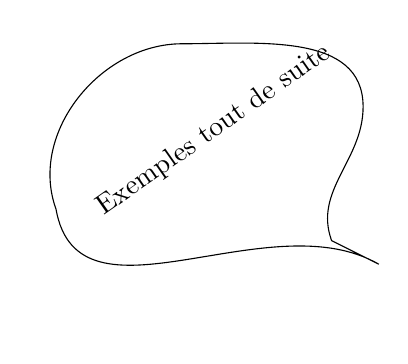
\begin{tikzpicture}
\node[rotate=35] (t) at (0,0) {\uline{Exemples \unsure{tout} de suite}};
\draw (-2,-1) to[out=110,in=180] (-.4,1.1)
to[out=0,in=90] (1.9,.3) to[out=-90,in=110] (1.5,-1.4)
--(2.1,-1.7) to[out=150,in=-80] (-2,-1);
\end{tikzpicture}}}

\margin{32}
\scanpage{34}

\uline{Remarque 1} La \uline{propriété $LG$ faible} \uline{équivaut}
à $(LG)_0$.

En effet, il suffit de prouver qu'elle implique que
\[
H^1(X,F)\longrightarrow H^1(X_{/Y},F_{/Y})
\]
est injectif, donc que tt. ext. de $\underline O_X$ par $F$
qui splitte formellement, splitte \unsure{régulièrement|réellement}, ce qui est immédiat.
[Question : si $\alpha$ est un isom pour $i\leq n$,
$\forall$ $F$ loc libre, est-il vrai que $\alpha$ est un mono
pour \deleted{tout} $i=n+1$, $\forall$ $F$ loc libre ?]
\inserted{Oui, prendre une \unsure{résolution} injective,
$0\longrightarrow F\longrightarrow I\longrightarrow G\longrightarrow0$
et \unsure{vérifier que le foncteur} $/Y$, \unsure{et la}
\unsure{limite} des $\unsure{G}=0$]}

\uline{Remarque 2}
Soit $(L_\alpha)$ une famille de Modules loc. libres sur $X$,
telle que $\forall$ module loc. libre sur $X$, est
$\simeq$ quotient d'une somme directe de Modules $\check L_\alpha$,
i.e. $\simeq$ sous-module \inserted{loc. facteur direct}
d'une somme directe de Modules $L_\alpha$.
[Ex : 1) $X$ quasi \deleted{\unsure{projectif}}\inserted{affine},
$(L_\alpha)$ réduit à $\underline O_X$
2) $X$ quasi-proj,
$(L_\alpha)$ formé des $\underline O(m)$, $m\geq m_0$].
Alors $(LG)_n$ équivaut à la condition
\[
H^i(X,L_\alpha)\simeq H^i(X_{/Y},L_{\alpha/Y})
\quad\left|\begin{array}{l}
\text{isom pour }i\leq n\\
\text{inj pour }i=n+1
\end{array}\right.
\]
\deleted{[N.B. \inserted{\unsure{Confiance} :}
\unsure{faut le prouver} \unsure{en mettant une}
condition sur $i=n+1$ !]}.
Dém par récurrence sur $n$, trivial si $n<-1$,
donc $\unsure{n+1<0|n\geq0}$, supposons \deleted{\unsure{on}}
que c'est prouvé

\margin{N.B. Le même argument marche si on
\unsure{ne l'exige que la} condition
$H^{\unsure{n+1|n}}(\unsure{L_\alpha})\longrightarrow
H^{\unsure{n+1|n}}(\unsure{\hat L_\alpha})$
\uline{injectif}.
\deleted{\unsure{Cet|Cat} \unsure{résultat|réserve}}}

\margin{33}
\scanpage{35}

pour les $i<n$. \deleted{Prouvons que} Nous savons donc déjà
que $(\unsure{\alpha})$ est bijectif pour $i\leq n-1$,
injectif pour $i=n$, on veut gagner un cran.
On a une suite exacte
\diagram{\begin{tikzcd}[column sep=small]
{}\arrow[r,dash] & F\arrow[r] & L\arrow[r] & G\arrow[r] &0
\end{tikzcd}}
où \inserted{$G$ loc libre,} $L$ est une somme directe de
modules loc. libres \deleted{\unsure{sommes}} $\simeq L_\alpha$,
donc les assertions à prouver sont vraies pour $L$.
Considérons l'hom de suites exactes
\diagram{\begin{tikzcd}[column sep=small]
H^i(L)\arrow[r,dash]\arrow[d,"\alpha"',"\sim"] &
H^i(G)\arrow[r,dash]\arrow[d,"\beta"] &
H^{i+1}(F)\arrow[r]\arrow[d,"\varphi"] &
H^{i+1}(L)\arrow[r,dash]\arrow[d,"\alpha'"',"\sim"] &
H^{i+1}(G)\arrow[d,"\beta'"] \\
H^i(\hat L)\arrow[r] & H^i(\hat G)\arrow[r] &
H^{i+1}(\hat F)\arrow[r,dash] & H^{i+1}(\hat L)\arrow[r] &
H^{i+1}(\hat G)
\end{tikzcd}}
pour $i=n-1,n$ donc $i+1=n,n+1$.
Dans le premier cas, on veut prouver que la flèche médiane
est surjective, dans le deuxième qu'elle est injective.

a) $i=n-1$, on sait par hyp. de réc. que $\beta$ est
surjective \deleted{(ou bijective)}
\deleted{il en est de même de $\alpha'$},
\inserted{de plus $\alpha'$ est surj par hyp.}
\deleted{\unsure{et puis par l'hyp. de réc.}}
\inserted{$\beta'$ est injective.}
Par lemme des 5, $\varphi$ est \deleted{bijective} surjective
\inserted{(donc bijective)}.

b) $i=n$, On sait par \deleted{a) \unsure{que}
\unsure{l'hyp} \unsure{pour} $\beta$}
récurrence que $\alpha$ et $\beta$ sont bijectives,
donc $\alpha$ est surj, $\beta$ inj, de plus $\alpha'$ est inj.

\margin{34}
\scanpage{36}

\uline{Remarque 3} Les conditions $LG$ et $LG$ effective sont
stables par passage de $X$ à un voisinage ouvert $U$ de $Y$.
Il n'en est plus de même en général des conditions $(LG)_n$,
\deleted{en particulier $(LG)_0$ \unsure{Cependant}
on peut prouver facilement qu'il en est encore ainsi de
$(LG)_0$, [et d'ailleurs]}
probablement pas même pour $(LG)_0$, en raison du fait
que un module loc. libre \inserted{$F$} sur un voisinage $U$
de $Y$ n'est pas restriction d'un module loc libre sur
\deleted{un voisinage} $X$.
Si cependant $\forall$ tel $F$ est isom. à un \uline{quotient}
d'un module loc. libre sur $X$ [p. ex. si $\forall$ Module
coh. sur $X$ est quotient d'un Module loc libre,
p. ex. $X$ quasi-projectif]]
\uline{alors} $(LG)_0$ pour $(X,Y)$ implique
$(LG)_{\unsure{n|0}}$ pour $\forall$ $(U,Y)$ i.e. $LG$ pour $(X,Y)$.
En effet on est ramené à prouver que pour $F$ loc libre
\uline{sur $X$},
\[
H^0(\unsure{U},F)\longrightarrow H^0(U_{/Y},F_{/Y})
\]
est bijectif, on sait déjà qu'il est surjectif,
[car
\diagram{\begin{tikzcd}[column sep=small]
H^0(X,F)\arrow[r,dash] & H^0(U,F)\arrow[r,dash] & H^0(U_{/Y},F_{/Y})
\end{tikzcd}}
l'est] reste à vérifier l'\uline{injectivité}, ce qui résulte de
\deleted{\unsure{pour}} \deleted{\unsure{donc que}}

\margin{35}
\scanpage{37}

$x\in U$, $\bar x^{(U)}\cap Y=\varnothing\ \Longrightarrow\
x\notin\operatorname{Ass}\underline O_X$, on conclut du

\uline{Lemme} Si $(Y,X)$ satisfait $(LG)_0$, alors pour
$\forall$ $x\in X$ tel que $Y\cap\bar x=\varnothing$,
on a $x\notin\operatorname{Ass}O_X$, du moins si $X$ est
quasi projectif.

\uline{Dém} Sinon, il existe un sous-faisceau coh $F$
\deleted{\unsure{de}} de $\underline O_X$
\deleted{\unsure{concentré}} de support $\bar x$.
Donc il existe une section non nulle de $F(n)\subset O_X(n)$,
[$n$ assez grand], \deleted{donc} \deleted{\unsure{qui}}
elle induira une section nulle de
$\underline O_{\deleted{\unsure{X}}}(n)_{/Y}$, absurde.

\fbox{\begin{minipage}{0.94\linewidth}
Conclusion pratique : Si $X$ quasi-projectif, alors
\diagram{\begin{tikzcd}[column sep=small,row sep=large,ampersand replacement=\&]
(LG)_0
\arrow[r,Leftarrow]
\arrow[r,Rightarrow,bend right=38,"\unsure{h}"'] \&
(LG)_{\text{faible}}
\arrow[r,Leftrightarrow]
\arrow[rr,Rightarrow,bend right=55,"\unsure{h}"'] \&
(LG)
\arrow[l,Rightarrow,bend left=38,"\unsure{h}"]
\arrow[r,Leftrightarrow] \&
\substack{H^0(X,\underline O_X(n))\xrightarrow{\sim}
H^0(X,\underline O_X(n)_{/Y})\\\text{pour }n\text{ grand}}
\end{tikzcd}}
\end{minipage}}

\margin{36}
\scanpage{38}

2) Premières propriétés [concernant $\pi_0$, $\pi_1$, Pic]

\uline{Proposition} Supposons que
$H^0(X,O_X)\mathbin{-}H^0(X_{/Y},O_{X/Y})$
soit injectif [bijectif] alors
$\pi_0(Y)\longrightarrow\pi_0(X)$ est surjectif [bijectif].
En particulier $(LG)_{-1}$ [resp $(LG)_0$] implique que
$\pi_0(Y)\longrightarrow\pi_0(X)$ est surjectif [bijectif].

\uline{Proposition} Supposons que $(X,Y)$ satisfasse
$LG$ (resp. $LG$ stricte).
\inserted{et $\unsure{\eta|\xi}$ un pt géom. de $Y$
(\unsure{connexe})}
Alors $\pi_1(Y)\mathbin{-}\pi_1(X)$ est surjectif [resp.
\[
\pi_1(Y,\unsure{\eta|\xi})\longrightarrow
\mathop{\mathrm{lim}}_{\substack{\longleftarrow\\
U\text{ voisinage}\\\text{ouvert de }Y}}
\pi_1(U,\unsure{\eta|\xi})
\]
est un hom \deleted{surjectif [resp.} bijectif]].

Résulte des faits plus généraux

\uline{\deleted{Corollaire}} \inserted{Lemme}
Supposons $LG$. \deleted{+ Alors \unsure{pour} $\forall$}
$F$ loc libre sur $X$;
(i) tt structure d'alg.
\deleted{[\unsure{resp.} \unsure{associative}, à unité, resp. commutative]}
\deleted{\unsure{connue}} sur $\hat F$ provient d'une structure
d'algèbre unique sur $F$, qui est ass (resp unitaire,
resp. comm.) ssi celle de $\hat F$ l'est.

\deleted{\unsure{de même que}}
\deleted{(ii) les décompositions de $F$ \deleted{\unsure{sont aussi}}
\inserted{en} produits de \inserted{deux} algèbres non nulles
correspondent aux décompositions analogues de $\hat F$
[\unsure{en liaison avec|en biject. avec} \unsure{celles de} $\unsure{F(n)|\Gamma(X)}$].}
Donc si $X'=\operatorname{Spec}(F)$, alors $X'$ connexe
ssi $\hat X'_{/Y}$ connexe

\margin{(iii) Un hom \inserted{$F\longrightarrow G$}
\deleted{de préschémas} de Modules munis de structures
d'alg. est un hom d'alg. ssi
$\hat F_{/Y}\longrightarrow G_{/Y}$ l'est.}

\margin{\deleted{\uline{Lemme}
[\unsure{L'immersion}, \unsure{la}\illegible{1}
dans un \unsure{voisinage} \unsure{de}\illegible{1}
\unsure{particulier} \unsure{fini} \unsure{ét.}
\unsure{donne} un foncteur \uline{pl. fidèle}
de catégories \unsure{étales|d'actions}]}}

\margin{37}
\scanpage{39}

D'où on conclut, utilisant l'équivalence de la catégorie
des rev. étales de $Y$ et des rev. étales de $X_{/Y}$, le

\uline{Corollaire} Si $(LG)$ vaut, alors le foncteur
$X'\longmapsto X'\times_XY$ des rev. étales de $X$ dans les
rev. étales de $Y$ est pleinement fidèle,
\deleted{Si $\unsure{X}$ $(LG)$ stricte vaut, pour}
et kif kif en remplaçant $\unsure{Y|X}$ par un voisinage
ouvert $U$ quelconque de $Y$.
Si $(LG)$ stricte vaut, alors pour tout rev étale $Y'$ de $Y$,
il existe un \deleted{rev étale $U'$ d'un}
voisinage ouvert $U$ de $Y$, et un rev. étale $U'$ de $U$,
\deleted{tel que} \inserted{\unsure{et d'un|et un}}
$Y$-isom $U'\times_UY\simeq Y'$.
(Si $U$ est choisi, $U'$ est bien déterminé à isom unique près).

\uline{Remarque}. Nous verrons plus loin des conditions,
liées au ``th de pureté'' permettant de conclure que
$\pi_1(U)\longrightarrow\pi_1(X)$ est
\deleted{surjectif}\inserted{bijectif}.
Kif-Kif pour Picard ---

\margin{38}
\scanpage{40}

\uline{Proposition} (i) Si $(LG)$ est satisfaite, alors pour
\deleted{$\forall$ voisinage ouvert}
$\operatorname{Pic}(X)\longrightarrow\operatorname{Pic}(X_{/Y})$
est injectif, et plus généralement, on a un hom injectif
\[
(\alpha)\qquad
\mathop{\mathrm{lim}}_{\substack{\longrightarrow\\U\supset Y}}
\operatorname{Pic}(U)\longrightarrow\operatorname{Pic}(X_{/Y})
\]
avec hom de transition injectifs.

(ii) Si $(LG)$ strict est satisfait, alors $\alpha$ est un isom.

\uline{Corollaire} Supposons que $Y$ ``est'' un diviseur de
Cartier sur $X$, soit $\deleted{\unsure{\mathcal O}}\Lambda\simeq
\underline L(Y)$ le faisceau inv. associé, donc
$i^*(\Lambda)^{-1}\simeq J/J^{\unsure{2}}$,
où $J$ est l'Idéal définissant $Y$.
[$i:Y\longrightarrow X$ désigne l'injection canonique.

\margin{introduire aussi les $Y_n$ pour exprimer ces propriétés}

(i) Supposons $H^1(Y,\Lambda^{-n})=0$ pour $n=1,2,\ldots$,
et $(LG)$. Alors $\operatorname{Pic}(X)\mathbin{-}\operatorname{Pic}(Y)$
est \uline{injectif}.
[\unsure{plus gén.} \deleted{\unsure{et on a les mêmes}}
\deleted{$(\alpha)$ est \unsure{injectif}}
les $\operatorname{Pic}(U)\longrightarrow\operatorname{Pic}(Y)$
sont injectifs, \unsure{donc} \deleted{\unsure{surjectifs}}
\unsure{de même}

(ii) Supposons
$\unsure{\deleted{H^1(Y,\Lambda^{-n})}|H^1(Y,\Lambda^{-n})}=0$
\uuline{et} $H^2(Y,\Lambda^{-n})=0$ pour $n=1,2,\ldots$,
et $(LG)$ strict.
Alors
\[
\mathop{\mathrm{lim}}_{\substack{\longrightarrow\\U\supset Y}}
\operatorname{Pic}(U)\simeq\operatorname{Pic}(Y).
\]

\margin{\[
\mathop{\mathrm{lim}}_{\substack{\longrightarrow\\U\supset Y}}
\operatorname{Pic}(U)\longrightarrow\deleted{\operatorname{Pic}(Y)}
\]
[et hom de transition injectifs]}

\margin{39}
\scanpage{41}

\deleted{Les \unsure{énoncés} \unsure{résultent}}
\inserted{La prop. résulte} aussitôt des
\deleted{\unsure{du} Lemme}\inserted{définitions, le}
Corollaire de la prop. et du

\uline{Lemme} : \deleted{\unsure{(i)}}
(i) Si $H^1(Y,\Lambda^{-n})=0$ pour $n=1,2,\ldots$,
alors \deleted{\unsure{pour} Pic} Le foncteur
$\unsure{\mathfrak F|\mathcal F}\longmapsto F_0$ des modules
\deleted{loc. libres} inversibles sur $\hat X$ dans les modules
inversibles sur $Y$ est pl. fidèle,
\deleted{\unsure{alors}} que
$\operatorname{Pic}(\hat X)\longrightarrow\operatorname{Pic}(Y)$
est injectif.

(ii) si de plus, $H^2(Y,\Lambda^{-n})=0$ pour $n=1,2,\ldots$,
alors le foncteur précédent est une équiv. de catégories,
donc $\operatorname{Pic}(\hat X)\longrightarrow\operatorname{Pic}(Y)$
est un isom.

3) \uline{Théorèmes de permanence}.

\deleted{
\uline{Théorème 1} Supposons que \deleted{si $X,Y$}
$(X,Y)$ satisfasse
\deleted{$(LG)_n$, et soit $f:X'\mathbin{-}X$ un}
\inserted{$(LG)_n$ et $X$ est quasi-projectif. Alors pour $\forall$}
morphisme \uline{projectif} et \uuline{plat},
\deleted{\unsure{alors}}
$f:X'\mathbin{-}X$, posant $Y'=f^{-1}(Y)$,
$(X',Y')$ satisfait $(LG)_n$.

\uline{\unsure{Th 2|Dém}} \uline{\unsure{Cas}}
Si $(X,Y)$ satisfait $(LG)$, alors
}

\unsure{\deleted{\uline{Pr. 2} Si $(X,Y)$ satisfasse $(LG)$
[resp. $(LG)$ effectif], \deleted{Alors} $X$ quasi-projectif,
-- alors}}

\margin{40}
\scanpage{42}

\deleted{pour tout $f:X'\mathbin{-}X$ \deleted{\unsure{plat}} \uline{projectif et plat},
posant $Y'=f^{-1}(Y)$, $(X',Y')$ satisfait $(LG)$
[resp. $LG$ stricte].}

\deleted{\uline{\unsure{Th 2}}}
\uline{Th} Soit $X$ \deleted{\unsure{pré}}schéma \deleted{\unsure{loc.}} noeth,
\inserted{quasi-projectif},
$Y$ partie fermée, $f:X'\longrightarrow X$ un morphisme
\uuline{quasi-projectif}, \inserted{$Y'=f^{-1}(Y)$. Soit}
$F'$ un faisceau coh. sur $X'$,
\uuline{plat} rel. /$\unsure{Y|X}$,
\inserted{à support propre sur $X$.}
Considérons les hom
\[
(\alpha)\qquad H^i(X',F')\longrightarrow H^i(X'_{/Y'},F'_{/Y'})
\]
\deleted{\unsure{les conditions}}.

\figure{\begin{tikzpicture}[x=1cm,y=1cm]
\draw (0,1.15) .. controls (-.6,.6) and (-.4,-.05) .. (.7,-.1)
 .. controls (3,-.22) and (7,-.2) .. (8.3,.25)
 .. controls (9,.6) and (9.2,1.15) .. (9,1.6)
 .. controls (7.6,2.05) and (5.5,1.95) .. (4.7,1.9);
\draw[->] (.8,-.1)--(.6,-.65);
\end{tikzpicture}}

(i) Si $(X,Y)$ satisfait $(LG)_n$, alors
$\alpha_i$ est un isom pour $i\leq n$, un \uline{mono.}
pour $i=n+1$.

(ii) Si $(X,Y)$ satisfait $(LG)$, alors pour
$\forall$ voisinage ouvert $U$ de $Y$, posant $U'=f^{-1}(U)$,
\deleted{\unsure{alors}} le foncteur
\deleted{\unsure{on}\quad $\forall$}
$F'\longmapsto F'_{/Y'}$
des Modules coh. sur $U'$ plats /$\unsure{Y|X}$
\inserted{et à support propre /$X$,}
\inserted{dans les Modules coh. sur $X'_{/Y'}$,}
plats sur $X_{/Y}=\mathfrak X$,
\inserted{(à support propre sur $\mathfrak X$),}
est pleinement fidèle.

\margin{$\operatorname{Hom}(F',G')\xrightarrow{\sim}
\operatorname{Hom}(F'_{/Y'},G'_{/Y'})$
pourvu que $\uuline{G'}$ soit plat sur $X$
[\unsure{pas la peine pour $F'$ dans la suite} $\ldots$]}

(iii) Si $(X,Y)$ satisfait $(LG)$ stricte, alors pour
$\forall$ Module coh. $\unsure{\mathfrak F'|F'}$ sur $X'_{/Y'}$, plat rel. $X_{/Y}$, il

\margin{41}
\scanpage{43}

existe un voisinage ouvert $U$ de $Y$, \deleted{\unsure{tel que}}
un module $F'$ sur $U'=f^{-1}(U)$, plat /$U$, et un
isom $F'_{/Y'}\simeq\unsure{\mathfrak F'|\mathcal F'}$.

\uline{Corollaire 2} Sous les conditions précédentes sur
$(X,Y)$, \inserted{(i) Si $(X,Y)$ satisfait $(LG)$,}
le foncteur $X'\longmapsto X'\times_X X_{/Y}$
de la catégorie des \deleted{pré}schémas \deleted{\unsure{loc.}} projectifs,
et plats sur $X$ dans la catégorie des
schémas formels projectifs et plats sur $X_{/Y}$
est pleinement fidèle. Kif Kif en
remplaçant $X$ par un voisinage ouvert $U$ de $Y$.

\margin{\unsure{peut se généraliser} aux schémas \uline{munis}
de faisceaux coh. \uline{rel. plats} et \uline{fidèles}.}

(ii) Si $(X,Y)$ satisfait $(LG\ \text{strict})$, pour
\deleted{tout} $\mathfrak X'$ \inserted{projectif de type fini}
\deleted{sur $\mathfrak X=X_{/Y}$}, plat sur $X_{/Y}$, il existe
un voisinage ouvert $U$ de $Y$, \deleted{\unsure{et}} un
$\unsure{U'}$ projectif \deleted{de type fini}
\inserted{et plat sur $U$,} et un
$\mathfrak X$-isom
\[
U'_{/Y'}\simeq\mathfrak X'\qquad (\unsure{\text{i.e.}|\div}\quad Y'=f^{-1}(Y)).
\]

\uline{Corollaire 1} \inserted{($X$ qu. projectif)}
\unsure{(i)} Si $(X,Y)$ satisfait $(LG)_n$
\deleted{\unsure{plat}}\inserted{[resp. $LG$, resp. $LG$ strict]},
alors pour $\forall$ $X'$ projectif et plat sur $X$,
posant \deleted{$\unsure{X}$} $Y'=f^{-1}(Y)$,
$(X',Y')$ satisfait $(LG)_n$.
\deleted{(ii) Si $(X,Y)$}
[resp. $(LG)$, resp. $(LG)$ stricte].

\margin{42}
\scanpage{44}

\uline{Remarque} On voit facilement par des exemples
dans le Th et les deux corollaires, que
les conditions de platitude et de \uline{propreté}
sont essentielles. Cependant, il \deleted{semble} est
possible que l'hypothèse de quasi-projectivité de
$X$ \deleted{et celle de}\inserted{de $X'$}
puisse être omise, \deleted{et celle
de propreté \unsure{puisse} \unsure{omise} dans le Th, et les
\unsure{premiers cas}},
\unsure{sans doute non plus dans}
cor. 2 (ii) [Existence d'un schéma
algébrique \unsure{donnant} un schém. formel].

\margin{43}
\scanpage{46}

\uline{Th.} $A$ anneau local noeth., quotient d'un régulier,
$t\in\mathfrak m_A$, $A$ \unsure{complet} pour la top. $t$-adique.
\[
X=\operatorname{Spec}(A),\quad Y=V(t),\quad x\ \text{cor. }\mathfrak m=\mathfrak m_A,
\qquad X'=X-\{x\},\quad Y'=Y-\{x\}=Y\cap X'.
\]
\[
\hat X=X_{/Y},\qquad \hat X'=X'_{/Y'},
\]
$\Phi$ l'ens. des parties fermées de $X'$,
ne rencontrant pas $Y'$, i.e. \uline{finies},
$C(X')$ la catégorie des faisceaux coh. sur $X'$,
$C_\Phi(X')$ la sous-catégorie des faisceaux à support $\in\Phi$.
Considérons le foncteur \inserted{\uline{exact}}
\[
F'\longmapsto\hat F'\ :\quad C(X')\mathbin{-}C(\hat X').
\]
Alors le foncteur est \uline{exact}, de \uline{noyau} $C_\Phi(X')$,
d'où définit un foncteur conservatif exact, : \unsure{a priori fidèle}
\[
\rho:\quad C(X')/C_\Phi(X')\longrightarrow C(\hat X').
\]
\unsure{]}

De plus, $\rho$ est \uline{pleinement fidèle}
\deleted{\illegible{2}} et
définit une \uline{équivalence de}
\inserted{$[C(X')/C_\Phi(X')]'$}
\uline{sur la catégorie des Modules coh. sur} $\hat X'$
\uline{qui sont} \deleted{\uline{restrictions}}
\inserted{\uline{\unsure{dominés|domiciliés}}}
\uline{de Modules coh. sur $\hat X$}, et
dont les \deleted{\unsure{composantes}}
\deleted{\unsure{de dimension} \unsure{support de dimension} $\unsure{\ne 1|+1}$}]
\inserted{\unsure{non nuls}}.

\margin{sur la sous-catégorie des
classes de $F'$ tels que \unsure{les} \unsure{dim.}
$\unsure{\overline{x}}\ \unsure{\ne2|\ge2}$
[\unsure{i.e. celles de $X'$} \unsure{de} $\unsure{t}$].
\inserted{\unsure{cycles associés à $F'$}}
\deleted{$\unsure{\dim\overline{x}}\ge2$ pour $\unsure{x\in X'}$}
\deleted{[\unsure{ne se prolonge pas} \illegible{2}
\uline{D.} \unsure{faisceaux} $\unsure{\operatorname{prof}F'_x}$
$\unsure{Y'}$, $\unsure{\dim}\ge3$]}}

\margin{Catégorie d'ailleurs \unsure{équivalente} à
la catégorie des $F'$ coh. sur $X'$
tels que $\operatorname{prof}F'_x\ge2$ pour
\deleted{$\unsure{x\in Y'}$}\inserted{$x\in X'-Y'$}
$\dim\overline{x}=1$, \uuline{et}
\deleted{$\operatorname{prof}F'_x\ne1$ \unsure{pour}}
\unsure{pas de cycles associés}
de dim $1\subset Y'$.}

Il faut surtout prouver que le foncteur
$\rho$ est \uline{pleinement fidèle}, ou encore ceci : si
$F',G'$ \deleted{sont} coh. sur $X'$ sont de prof $\ge2$ aux
pts \deleted{$x\in\Phi$ $\unsure{x}$ \unsure{de}}
fermés $x$ de $X'-Y'$, \deleted{\unsure{tout}} alors
\[
\operatorname{Hom}(F',G')\simeq\operatorname{Hom}(\hat F',\hat G').
\]
Pour en \unsure{revenir là}, \unsure{considérant}
$H=\underline{\operatorname{Hom}}(F,G)$,
on est ramené à prouver que
\[
\Gamma\unsure{F'}\simeq\Gamma\unsure{\hat F'}
\]
si $F'$ est de prof $\ge\unsure{2|3}$ aux pts
\inserted{fermés} de $X'-Y$.

\margin{45}
\scanpage{47}

II\hfill\mspage{- 11 -}\hfill n$^\circ$338

A tout $A$-module $M$, projectif de rang 1, faisons correspondre un élément
$J$ de $\underline I$ isomorphe à $M$ (prop.5), et notons $\operatorname{Cl}(M)$ l'image canonique de $J$ dans
$\underline I/\underline P$ ; comme deux idéaux fractionnaires isomorphes (en tant que $A$-modules)
sont homothétiques, $\operatorname{Cl}(M)$ est indépendant du choix de $J$. Pour que deux
$A$-modules $M$ et $M'$ projectifs, de type fini, et de rang 1 soient \uline{isomorphes},
il faut et il suffit que les éléments $\operatorname{Cl}(M)$ et $\operatorname{Cl}(M')$ soient \uline{égaux}. Comme
le produit tensoriel de deux modules projectifs est un modules projectif, et
donc sans torsion, il résulte de ce qui a été vu au début du n$^\circ$ que la multiplication
dans le groupe $\underline I/\underline P$ correspond au \uline{produit tensoriel} des $A$-modules
projectifs de rang 1. On dit parfois que $\underline I/\underline P$ est le groupe des $A$-modules
projectifs de rang 1.

\begin{center}\texttt{-:-:-:-:-}\end{center}

\margin{46}
\scanpage{48}

Pour le voir, on est ramené par un
dévissage facile, [utiliser l'existence d'une suite exacte
\diagram{\begin{tikzcd}[column sep=small]
0\arrow[r,dash]&P'\arrow[r,dash]&F'\arrow[r,dash]&\widetilde F'\arrow[r,dash]&Q'\arrow[r,dash]&0
\end{tikzcd}}
où $\operatorname{supp}P'\subset Y'$, $\operatorname{supp}Q'\subset Y'$,
$\dim\operatorname{supp}P'\leq0$, $\dim\operatorname{supp}Q'\leq1$,
et $\operatorname{prof}\unsure{\hat F'_{x'}|\widetilde F'_{x'}}$
\unsure{aux} $\forall$ pts fermés de $X'$ -- pas seulement de
$X'-Y'$] -- dévissage qui est une question purement locale
sur le schéma de \uline{Jacobson} $X'$] au cas où on a
$\operatorname{prof}F_x\ge2$, \deleted{D'ailleurs, si}
pour \uline{$\forall$ $x\in X'$}. Soit
d'ailleurs $K'$ le noyau de la multiplication par
\deleted{\unsure{sur $F_x$}}
$t^n$ ($n$ grand) on a
\diagram{\begin{tikzcd}[column sep=small]
0\arrow[r,dash]&K'\arrow[r,dash]&F'\arrow[r,dash]&C'\arrow[r,dash]&0
\end{tikzcd}}
\deleted{avec $C'$} $t$ \deleted{est} $C'$-régulier. On a

\margin{\figure{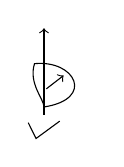
\begin{tikzpicture}[x=1cm,y=1cm]
\draw[->] (0,0)--(0,1.1);
\draw (0,.1) .. controls (.65,.2) and (.4,.7) .. (-.12,.65)
 .. controls (-.2,.4) and (0,.2) .. (0,.1);
\draw[->] (.03,.33)--(.25,.5);
\draw (-.2,-.1)--(-.1,-.3)--(.2,-.08);
\end{tikzpicture}}}

\margin{\figure{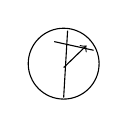
\begin{tikzpicture}[x=1cm,y=1cm]
\draw (0,0) ellipse (.45 and .45);
\draw (0,-.43)--(.05,.42);
\draw (-.12,.28)--(.38,.17);
\draw[->] (0,-.05)--(.29,.23);
\end{tikzpicture}}}

\diagram{\begin{tikzcd}[column sep=small,row sep=large]
&0\arrow[r,dash]&\Gamma K'\arrow[r]\arrow[d,"\sim"']&
\Gamma F'\arrow[r,dash]\arrow[d]&\Gamma C'\arrow[r,dash]\arrow[d,"\sim?"']&
H^1\unsure{K'|C'}\arrow[d,phantom,"\rotatebox{90}{$\simeq$}"]\\
A\quad\unsure{\hat A_\Phi|\hat A_\varphi}&0\arrow[r,dash]&\Gamma\hat K'\arrow[r,dash]&
\Gamma\hat F'\arrow[r,dash]&\Gamma\unsure{\hat C'|\hat G'}\arrow[r,dash]&H^1\unsure{\hat K'|\hat C'}
\end{tikzcd}}

On est ramené au cas où $t$ est \unsure{non} div. de $0$.

\figure{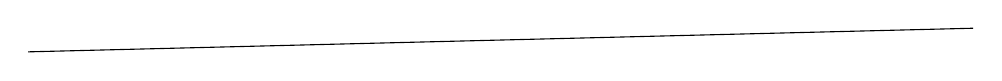
\begin{tikzpicture}\draw (0,0)--(12,.3);\end{tikzpicture}}

\margin{47}
\scanpage{49}

II\hfill\mspage{- 10 -}\hfill n$^\circ$338

que $\displaystyle\sum_{i=1}^n x_ix'_i=1$. Les applications $A$-linéaires
$f:(a_i)\longrightarrow\displaystyle\sum_{i=1}^n a_ix_i$ de $A^n$
dans $J$ et $g:y\longrightarrow(x'_iy)$ de $J$ dans $A^n$ sont telles que
$f\circ g$ est l'application identique de $J$. Donc $g$ est un isomorphisme de $J$
sur un facteur direct du module libre $A^n$ (\uline{Alg.} VIII,\S1, n$^\circ$1 ), ce qui montre que $J$ est projectif.

Réciproquement supposons $J$ projectif. Il existe alors un isomorphisme $f$
de $J$ sur un facteur direct $M$ d'un $A$-module libre $A^{(I)}$ ; notons $g$ la surjection
de $A^{(I)}$ sur $J$ obtenue en composant la projection de $A^{(I)}$ sur $M$ avec
l'isomorphisme $f^{-1}$. Soit $(e_i)_{i\in I}$ la base canonique de $A^{(I)}$ ; posons
$x_i=g(e_i)$. L'application $\operatorname{pr}_i\circ f$ de $J$ dans $A$ est $A$-linéaire, et il existe
donc un élément $x'_i$ du corps des fractions $K$ de $A$ tel que $\operatorname{pr}_i(f(x))=x'_ix$
pour tout $x\in J$, (lemme 6). Pour $x\in J$ donné, les éléments $x'_ix$ ($i\in I$) sont
nuls sauf un nombre fini d'entre eux ; comme $J\ne(0)$, on peut prendre $x\ne0$,
ce qui montre que les $x'_i$ sont nuls sauf un nombre fini d'entre eux. D'autre
part, comme $g\circ f$ est l'application identique de $J$, on a
$x=\displaystyle\sum_{i\in I}xx'_i\,x_i$ pour
tout $x\in J$. Prenant $x\ne0$, on en déduit $1=\displaystyle\sum_{i\in I}x'_ix_i$.
Comme $g$ est surjectif, on a $J=\displaystyle\sum_{i\in I}Ax_i$.
D'autre part il résulte aussitôt de ce qu'on a vu
que l'idéal fractionnaire $J'=\displaystyle\sum_{i\in I}Ax'_i$ est l'inverse de $J$.
Ainsi $J$ est inversible, ce qui achève la démonstration.

Il résulte des prop. 5 et 3 qu'un $A$-module projectif de rang 1 est
nécessairement de type fini.

\margin{\unsure{?}}
Soit toujours $A$ un anneau
\figure{
\begin{tikzpicture}[baseline=(w.base)]
\node[inner sep=0] (w) {intègre.};
\draw (.15,.12) .. controls (.15,.65) and (.7,.22) .. (.55,-.15)
 .. controls (.05,-.5) and (-.1,.1) .. (.15,.12);
\end{tikzpicture}}
L'ensemble $\underline I$ des idéaux fractionnaires
inversibles de $A$, muni de la multiplication, est un \uline{groupe commutatif} ;
l'ensemble $\underline P$ des idéaux fractionnaires principaux non nuls de $A$ est un sous-groupe
de $\underline I$. Le groupe quotient $\underline I/\underline P$ s'appelle le \uline{groupe des classes d'idéaux
de} $A$.

\margin{48}
\scanpage{50}

\deleted{\unsure{On considère} \illegible{1}}

\uline{Avec} cor. \unsure{3} du th. de comparaison affine

Supposons que $\unsure{\mathfrak F'|\mathcal F'}$ satisfasse a) b) c')
[c') est que $\unsure{\mathfrak F'|\mathcal F'}$ s'étende en un
$\unsure{\mathfrak F|\mathcal F}$ coh. sur $\hat X$], \unsure{je}
dis que $\unsure{\mathfrak F'|\mathcal F'}$ provient d'un $F'$ satisfaisant la
condition $\operatorname{prof}F'_x\ge2$ si $x\in T_1$.
En effet,
il provient déjà d'un $F'$ coh. \deleted{\unsure{tel que}}\inserted{où}
$t$ est $F'$-régulier, il faut au besoin modifier $F'$.

\deleted{Soit
$Z'$ l'ens. des pts de $\unsure{X'}$ tels que
$\operatorname{prof}_{x'}(F')\leq1$,
c'est une partie \deleted{constructible \unsure{et} \illegible{3}}
\inserted{fermée de $X'-Y'$}.
On peut déjà \unsure{supposer} en
\unsure{effet} que pour $\forall$ $x'\in\operatorname{Ass}F'$, on ait
\deleted{$\unsure{x'\notin Y'}$ $\unsure{\dim\overline{x'}\in T_1}$}
\unsure{i.e.} $\overline{x'}\cap Y'\ne\varnothing$, \unsure{quitte à}
\unsure{limiter} $\uline{F'}$ \unsure{à un ouvert convenable}.
\unsure{Considérons} l'ensemble $U$ des
$x'\in X'$ tels que $\operatorname{prof}_{x'}(F')\ge2$.}

\margin{adhérence $\overline{x'}$ dans $X'$}

\margin{On suppose $X$ \unsure{localisé}
autour de $T$, et
$X-T=X'$ \deleted{\unsure{partie}}\inserted{un}
\deleted{\illegible{2}}
\uline{Jacobson} ``\unsure{sympathique}''}

Si $x'$ est
un pt \uline{fermé} de \deleted{$\unsure{X}$} $Y'$, on a : par hyp.
$x'\in U$, c'est donc vrai pour $\forall$ pt de $Y'$,
donc $U$ est un \uline{voisinage} de $Y'$ dans $X'$.

\deleted{Je dis que $x'\in X'-U$ implique que}
Les pts de $X'-U$ sont donc \uline{fermés} dans $X'$
[et sont en fait dans $T_1$] -- ils sont à
fortiori en nbre fini. Soit $x'\in X'-U$, et
\uline{soit} \deleted{$x'_1\in\operatorname{Ass}F'$ \unsure{tel}}
$x'_1\in U$ tel que $x'_1\in\operatorname{Ass}F'$,
$\overline{x'_1}\ni x'$, je dis que \unsure{il n'est pas possible que}
$x'_1\uline{\unsure{\rightsquigarrow|\ne}}x'$ : sinon en effet, $\overline{x'_1}$ serait de dim $1$,

\margin{49}
\scanpage{51}

\mspage{- 134 -}\hfill n$^\circ$ 371

\S7. \uuline{Algèbre extérieure d'un espace vectoriel.}

1. \uline{Application des déterminants aux équations linéaires sur un corps commutatif.}

Les résultats des \S\S\ 5 et 6 donnent en particulier les suivants pour les
espaces vectoriels :

PROPOSITION 1.- \uline{Soit} $E$ \uline{un espace vectoriel sur un corps commutatif} ; \uline{pour que} $p$
\uline{vecteurs} $x_i$ ($1\leq i\leq p$) \uline{de} $E$ \uline{forment un système libre, il faut et il suffit que}
\[
x_1\wedge x_2\wedge\ldots\wedge x_p\ne0.
\]

C'est un cas particulier du \S6, n$^\circ$5, prop.7, tout élément $\ne0$ d'un corps étant
inversible.

COROLLAIRE 1.- \uline{Soit} $\underline X$ \uline{une matrice de type} $(m,n)$ \uline{sur un corps commutatif. Le rang
de} $\underline X$ \uline{est égal au plus grand des entiers} $p$ \uline{tels qu'il existe au moins un mineur
d'ordre} $p$ \uline{de} $\underline X$ \uline{qui ne soit pas nul.}

En effet, $\operatorname{rg}(\underline X)$ est le nombre maximum des colonnes de $\underline X$ linéairement indépendantes
(chap.II, 3e éd., \S10, n$^\circ$\quad ) ; le corollaire résulte donc de la prop.1 et de
l'expression des composantes d'un $p$-vecteur décomposable (\S6, n$^\circ$3, prop.5).

COROLLAIRE 2.- \uline{Pour qu'une matrice carrée sur un corps commutatif soit inversible,
il faut et il suffit que son déterminant ne soit pas nul.}

COROLLAIRE 3.- \uline{Pour qu'un système linéaire} homogène \uline{de} $n$ \uline{équations à} $n$ \uline{inconnues
sur un corps commutatif admette une solution non triviale, il faut et il suffit que
le déterminant de sa matrice soit nul.}

Considérons un système de $m$ équations linéaires à $n$ inconnues sur un corps commutatif $K$ :
\[
(1)\qquad\sum_{j=1}^n\alpha_{ij}\xi_j=\beta_i\qquad(1\leq i\leq m).
\]
La matrice $\underline A=(\alpha_{ij})$ de ce système est donc de type $(m,n)$. Soit $\underline B$ la matrice
de type $(m,n+1)$ obtenue en \uline{bordant} $\underline A$ par la $(n+1)$-ème colonne $(\beta_i)$ ; on sait

\margin{\rotatebox{180}{50}}
\scanpage{52}

donc \unsure{en les} pts fermés $z'$ de $\overline{x'_1}\cap U$, on
aurait $\operatorname{prof}F'_{z'}\leq1$, ce qui est absurde. Donc
si $i:U\mathbin{-}X'$ est l'inclusion, $F'_1=i_*(F'|U)$
est cohérent, et évidemment de prof $\ge2$
sur $X'-U$, d'autre part il est de prof $\ge2$
aux pts fermés de \deleted{$\unsure{X}$} $U$, donc
$F'_1$ est de prof $\ge2$ en \uline{$\forall$} pt fermé de $X'$,
on a gagné.

\margin{51}
\scanpage{53}

\mspage{- 133 -}\hfill n$^\circ$371

$n-2$ \uline{de} $\underline X$ \uline{obtenu en supprimant dans} $\underline X$ \uline{les lignes d'indices} $i$ \uline{et} $j$ \uline{et les colonnes
d'indices} $h$ \uline{et} $k$ ; \uline{on a alors}
\[
(38)\qquad X^{ih}X^{jk}-X^{ik}X^{jh}=(\det\underline X).X^{ij,hk}.
\]
Il suffit d'appliquer la formule (35) lorsque $H=I-\{i,j\}$, $K=I-\{h,k\}$,
où $I=\unsure{[\![1,n]\!]|[1,n]}$.

Nous verrons au chap.IV que les formules (34) à (38) sont encore
valables sans aucune hypothèse sur la matrice carrée $\underline X$.

\begin{center}\texttt{-:-:-:-:-}\end{center}

\margin{\rotatebox{180}{52}}
\scanpage{54}

\unsure{Applications} aux morphismes
\uline{\deleted{\unsure{hyperplans|projectifs}} projectifs}
et aux morphismes propres

\margin{53}
\scanpage{56}

\figure{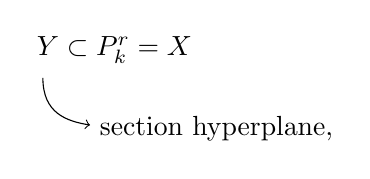
\begin{tikzpicture}[x=1cm,y=1cm]
\node[anchor=west] at (0,1) {$Y\subset P^r_k=X$};
\node[anchor=west] at (.8,0) {section hyperplane,};
\draw[->] (.2,.65) .. controls (.2,.2) and (.5,.1) .. (.8,.05);
\end{tikzpicture}}
$U$ voisinage de $Y$, $Z=X-U$
\inserted{ens. \unsure{fermé|fini} fini}

$F$ cohérent sur $X$

a) Condition pour que $H^i(U,F(-m))=0$ pour $m$ grand?

\unsure{a')|d)} Condition pour que
$\unsure{\coprod_m|\bigoplus_m}H^i(U,F(m))$ de type fini sur $S$

b) Condition pour que $H^i(U,F(m))=0$ pour $m$ grand

($i>0$ donné)

\unsure{c)} Condition pour que
\[
H^i(U,F)\longrightarrow H^i(\hat X,\hat F)
\]
soit un isomorphisme?

\figure{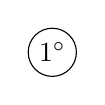
\begin{tikzpicture}\node[draw,circle,inner sep=2pt] {$1^\circ$};\end{tikzpicture}}
Considérons la suite exacte
(où $E^d=\underline{\operatorname{Ext}}^d_{O_X}(F,\omega_X)$)

\diagram{\begin{tikzcd}[column sep=small,row sep=large]
H^i_Z(X,F(\unsure{-m}))\arrow[r,"\alpha_i"]&
H^i(X,F(\unsure{-m}))\arrow[r]&
H^i(U,F(\unsure{-m}))\arrow[r]&
H^{i+1}_Z(X,F(\unsure{-m}))\arrow[r,dash,"\alpha_{i+1}"]&
H^{i+1}(X,F(-m))\\
\prod_{z\in Z}\bigl(E^{r-i}(m)\bigr)^\wedge_z&
\Gamma E^{r-i}(m)\arrow[l]&&
\prod_{z\in Z}\bigl(E^{r-i-1}(m)\bigr)^\wedge_z&
\Gamma E^{r-i-1}(m)\arrow[l]
\end{tikzcd}}

Conditions équivalentes

\diagram{\begin{tikzcd}[row sep=large]
\alpha_i\ \text{surjectif pour }m\text{ grand}
\quad\deleted{\text{\unsure{pour tout $m$}}}
\arrow[d,Leftrightarrow]\arrow[dd,bend right=65]\quad\\
z\in Z\ \Rightarrow\ z\text{ isolé dans }(\operatorname{supp}E^{r-i}\cup\{z\})
\arrow[d,Leftrightarrow]\\
H^{i-1}(X,F(-m))\longrightarrow H^{i-1}(U,F(-m))
\quad\text{\uline{surjectif} pour }m\text{ grand}
\end{tikzcd}}

\margin{\unsure{*}}
\diagram{\begin{tikzcd}[row sep=large]
\alpha_i\ \text{injectif pour }m\text{ grand},\quad i\leq n\quad\Longleftrightarrow
\arrow[d,Leftrightarrow]\\
\exists\text{ voisinage ouvert }V\text{ de }Z,\text{ tel que }F
\text{ soit de profondeur }>n\text{ sur }U\cap V
\arrow[d,Leftrightarrow]\\
H^i(X,F(-m))\mathbin{-}H^i(U,F(-m))\quad
\text{surjectif pour }m\text{ grand},\ i<n
\end{tikzcd}}

\figure{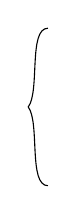
\begin{tikzpicture}[x=1cm,y=1cm]
\draw (.25,2) .. controls (0,2) and (.15,1.2) .. (0,1)
 .. controls (.15,.8) and (0,0) .. (.25,0);
\end{tikzpicture}}

\margin{55}
\scanpage{57}

$F_0$ le Module qu'il induit sur $X_0$. On suppose a) Pour tout $s\quad S$,
la section $t_s$ induite par $t$ sur la fibre $X_s$ est
$\underline O_{X_s}$-régulière et $\underline F_s$-régulière
b) $\underline F$ et $\underline O_X$ sont plats par rapport à $S$
c) Pour tout $s\quad S$, $F_{0\,s}$, \deleted{et}
$\underline O_{X_{0\,s}}$ \inserted{et $\underline O_X$}
sont de profondeur $\quad 2$ en les points fermés de
$X_s\deleted{\unsure{s|z}}$.
Sous ces conditions, il existe un Module cohérent $F$ sur $X$, et un isomorphisme
de son complété formel $\hat F$ le long de $X_0$ avec $\underline F$.

Cet énoncé va résulter du suivant:

\uline{Corollaire} 3.2.\quad Sous les conditions de \unsure{3.1}.\quad (

\[
\coprod_{\substack{p\unsure{\gg|\ge}0\\q\geq0}}F_0(q-p)
\]
\[
M+M(1)+\cdots+M(-p)
\qquad
\coprod_{\unsure{0},q}S_q
\]

\figure{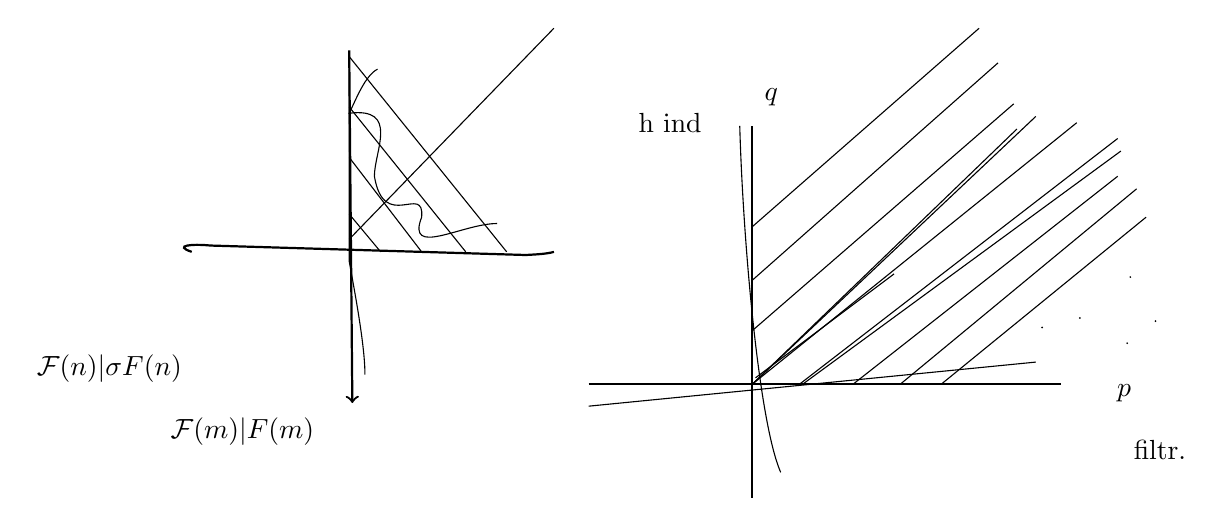
\begin{tikzpicture}[x=.8cm,y=.8cm]
\draw[thick] (-2.5,0) .. controls (-2.8,.1) and (-2.5,.13) .. (-2.2,.1)
 -- (2.8,-.05) .. controls (3,-.04) and (3.15,-.03) .. (3.25,0);
\draw[thick,->] (0,3.2) -- (.05,-2.4);
\draw[thin] (0,2.9) -- (0,-.15) .. controls (.1,-.7) and (.25,-1.5) .. (.25,-1.95);
\draw (0,3.1) -- (2.5,0);
\draw (0,2.3) -- (1.85,0);
\draw (0,1.5) -- (1.15,0);
\draw (0,.6) -- (.5,0);
\draw[thin] (0,.2) -- (3.25,3.55);
\draw[thin] (.45,2.9) .. controls (.25,2.8) and (.1,2.4) .. (0,2.2)
 .. controls (.8,2.3) and (.4,1.6) .. (.4,1.2)
 .. controls (.55,.3) and (1.2,1.1) .. (1.15,.55)
 .. controls (.9,-.1) and (1.8,.45) .. (2.35,.45);
\node[anchor=east] at (-2.5,-1.85) {$\unsure{\mathcal F(n)|\sigma F(n)}$};
\node[anchor=east] at (-.4,-2.85) {$\unsure{\mathcal F(m)|F(m)}$};
\begin{scope}[shift={(6.4,-2.1)}]
\draw[thick] (-2.6,0) -- (4.9,0);
\draw[thick] (0,-1.8) -- (0,4.1);
\draw[thin] (-.2,4.1) .. controls (-.15,2.3) and (.1,-.6) .. (.45,-1.4);
\draw[thin] (-2.6,-.35) -- (4.5,.35);
\draw (0,2.5) -- (3.6,5.65);
\draw (0,1.65) -- (3.9,5.1);
\draw (0,.85) -- (4.15,4.45);
\draw (0,0) -- (4.5,4.25);
\draw[thin] (0,0) -- (4.2,4.05);
\draw (0,0) -- (5.15,4.15);
\draw[thin] (.05,.1) -- (2.25,1.75);
\draw (.75,0) -- (5.8,3.9);
\draw[thin] (.8,0) -- (5.85,3.7);
\draw (1.6,0) -- (5.8,3.3);
\draw (2.35,0) -- (6.1,3.1);
\draw (3,0) -- (6.25,2.65);
\node at (.3,4.55) {$q$};
\node at (5.9,-.15) {$p$};
\node[anchor=east] at (-.65,4.15) {\unsure{h ind}};
\node[anchor=west] at (5.9,-1.05) {\unsure{filtr.}};
\fill (5.2,1.05) circle (.015);
\fill (6,1.7) circle (.015);
\fill (6.4,1) circle (.015);
\fill (5.95,.65) circle (.015);
\fill (4.6,.9) circle (.015);
\end{scope}
\end{tikzpicture}}

\diagram{\begin{tikzcd}
H^i(X,F)\arrow[r]&H^i(\hat X,\hat F)
\end{tikzcd}}

\margin{56}
\scanpage{58}

\diagram{\begin{tikzpicture}
\node[anchor=north west,inner sep=0pt] (g) at (0,0) {\begin{tikzcd}[row sep=large]
\alpha_i\text{ bijectif pour }m\text{ grand}\arrow[d,Leftrightarrow]\\
\operatorname{Supp}E^{r-i}\subset Z\arrow[d,Rightarrow]\\
H^i_x(F_x)=0\quad\text{pour }\forall\ x\text{ fermé \uline{en $U$}.}
\end{tikzcd}};
\draw (g.north west) .. controls +(-.3,0) and +(-.2,.3) .. (g.west)
 .. controls +(-.2,-.3) and +(-.3,0) .. (g.south west);
\end{tikzpicture}}

\diagram{\begin{tikzpicture}
\node[anchor=north west,inner sep=0pt] (g) at (0,0) {\begin{tikzcd}[row sep=large]
\alpha_i\text{ bijectif pour }m\text{ grand},\quad i\leq n\arrow[d,Leftrightarrow]\\
\operatorname{supp}E^{r-i}\subset Z\quad\text{pour }i\leq n\arrow[d,Leftrightarrow]\\
\operatorname{prof}(F_x)>n\quad\text{pour }\forall\ x\text{ fermé \uline{en} }U
\arrow[d,Leftrightarrow]\\
\begin{gathered}
H^i(U,F(-m))=\deleted{H^{\unsure{0|i}}(\unsure{X|U},F(-m))}
\inserted{0\quad\text{pour }m\text{ grand},\ i<n\quad\text{\uuline{et}}}
\quad\deleted{\text{bijectif pour }i\leq n}\\
H^n(U,F(-m))\longrightarrow H^{n+1}_{\inserted{Z}}(X,F(-m))
\quad\deleted{\text{surjectif pour }i\leq n}\ \inserted{\text{injectif}}
\end{gathered}
\end{tikzcd}};
\draw (g.north west) .. controls +(-.3,0) and +(-.2,.35) .. (g.west)
 .. controls +(-.2,-.35) and +(-.3,0) .. (g.south west);
\end{tikzpicture}}

\diagram{\begin{tikzpicture}
\node[anchor=north west,inner sep=0pt] (g) at (0,0) {\begin{tikzcd}[row sep=large]
\begin{gathered}
\alpha_i\text{ bijectif pour }m\text{ grand},\quad i\leq n\\
\text{et }\alpha_i\text{ injectif pour }m\text{ grand},\quad i=n+1
\end{gathered}\arrow[d,Leftrightarrow]\\
\begin{gathered}
\deleted{\unsure{\operatorname{prof}}}\ \operatorname{supp}E^{r-i}\subset Z
\quad\text{pour }i\leq n,\quad\operatorname{supp}E^{r-n-1}\ \text{\unsure{ne peut}}\\
\text{\unsure{avoir un pt de $Z$ pour}}\ \text{\illegible{2}}\ \text{\unsure{pts isolés}}
\end{gathered}\arrow[d,Leftrightarrow]\\
\begin{gathered}
\operatorname{prof}(F_x)>n\text{ si }x\text{ fermé en }U,\quad\text{et}\\
\operatorname{prof}(F_x)>n+1\text{ si de plus }x\in V\cap U,\quad V\text{ voisinage}\\
\text{ouvert convenable de }Z
\end{gathered}\arrow[d,Leftrightarrow]\\
H^i(U,F(-m))=0\quad\text{pour }m\text{ grand},\quad i\leq n\arrow[d,Leftrightarrow]\\
\coprod_{m\unsure{\geq|\gg}0}H^i(U,F(m))\text{ de type fini sur }S(\unsure{-h})\quad i\leq n
\end{tikzcd}};
\draw (g.north west) .. controls +(-.4,0) and +(-.25,.5) .. (g.west)
 .. controls +(-.25,-.5) and +(-.4,0) .. (g.south west);
\node[draw,circle] at (-1.2,-3) {$B_n$};
\node[draw,ellipse,align=center] (m) at (-2,-7.1)
 {$H^i(U,F)$\\de dim finie\\pour $i\leq n$};
\draw[->,double] (-.2,-6.65) -- node[above] {cf $2^\circ$} (m.north east);
\end{tikzpicture}}

Cela \unsure{résout} la question (a). Sous les conditions de (*), on a donc
[si $t$ est $F$-régulier]
\[
\left\{\begin{gathered}
H^i(U,F)\overset{\sim}{\longrightarrow}H^i(\hat X,\hat F)
\quad\text{est}\quad
\begin{cases}\text{iso si }i<n\\\text{mono si }i=n\end{cases}\\
H^i(\hat X,\hat F)\simeq\varprojlim H^i(X_m,F_m)\quad\text{pour }i\leq n
\end{gathered}\right.
\]

\margin{57}
\scanpage{59}

Ce qui donne des conditions suffisantes pour la validité de c).
Cependant, elles ne sont pas nécessaires [même en exigeant la validité de c
pour $i<n$, et tous les tordus de $F$], comme on voit en faisant $n=1$:
car il suffit qu'on ait $\operatorname{prof}F_x\geq2$ pour $x$ fermé en $U$,
pour pouvoir conclure que
\[
H^0(U,F)\unsure{\mathbin{-}|\longrightarrow}H^0(\hat X,\hat F)
\]
est bijectif.

\figure{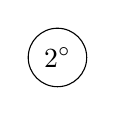
\begin{tikzpicture}\node[draw,circle] {$2^\circ$};\end{tikzpicture}}
La suite exacte nous apprend que \unsure{l'hom.}
\[
H^i(U,F)\longrightarrow H^{i+1}_Z(X,F)
\]
est un isom mod \unsure{vectoriels} finis. donc

\deleted{$H^i(U,F$}

\diagram{\begin{tikzpicture}
\node[anchor=north west,inner sep=0pt] (g) at (0,0) {\begin{tikzcd}[row sep=large]
H^i(U,F)\text{ de dim finie sur }k\arrow[d,Leftrightarrow]\\
H^{i+1}_z(F_z)\text{ de dim finie (i.e. de long. \unsure{finie}]}\quad
\text{pour }\forall\ z\in Z\arrow[d,Leftrightarrow]\\
z\unsure{\in}Z\Longrightarrow z\text{ pt isolé de }\operatorname{supp}E^{r-i-1}\cup\{z\}
\arrow[d,Leftrightarrow]\\
\alpha_{i+1}\text{ injectif pour }m\text{ grand}\arrow[d,Leftrightarrow]\\
H^i(X,F(m))\mathbin{-}H^i(U,F(\unsure{-m|m}))\quad\text{surjectif pour }m\text{ grand}
\end{tikzcd}};
\draw (g.north west) .. controls +(-.4,0) and +(-.2,.4) .. (g.west)
 .. controls +(-.2,-.4) and +(-.4,0) .. (g.south west);
\node[draw,circle] at (-1,-2.7) {$A'_i$};
\end{tikzpicture}}

\margin{58}
\scanpage{60}

\margin{$R^p\unsure{f|j}_*[R^qg_*(\unsure{F\deleted{(m)}|\deleted{F(m)}}))$}

\deleted{\[
H^i(U,F(m))\longrightarrow H^i_{\unsure{Y|Z}}
\]}

\deleted{\diagram{\begin{tikzpicture}
\node[anchor=north west,inner sep=0pt] (g) at (0,0) {\begin{tikzcd}[row sep=large]
H^i(U,F(m))\arrow[d,Leftrightarrow]\\
\coprod_{m\geq0}H^i(U,F(m))\text{ de type fini sur }S\quad\text{pour }i\leq n
\arrow[d,Leftrightarrow]\\
\begin{gathered}
R^ig_*(F)\text{ coh. pour }i\leq n,\text{ i.e. }\underline H^i_Z(F)\text{ coh pour }i\leq n+1\\
\text{i.e. }H^i_z(F_z)\text{ de dim finie pour }i\leq n+1,\ z\in Z
\end{gathered}
\end{tikzcd}};
\draw (g.north west) .. controls +(-.3,0) and +(-.25,.4) .. (g.west)
 .. controls +(-.25,-.4) and +(-.3,0) .. (g.south west);
\node at (-.7,-1.1) {$3^\circ$};
\draw (-1.5,-.8) -- (12,-.8);
\draw (g.south west) -- (g.south east);
\end{tikzpicture}}}

\diagram{\begin{tikzpicture}
\node[anchor=north west,inner sep=0pt] (g) at (0,0) {\begin{tikzcd}[row sep=large]
H^i(U,F)\text{ de dim finie si }i\leq n\arrow[d,Leftrightarrow]\\
F\text{ de prof }>n+1\text{ sur }U\text{ au voisinage de }Z\arrow[d,Leftrightarrow]\\
z\in Z\Longrightarrow z\text{ pt isolé de }\operatorname{supp}E^{r-i-1}\cup\{z\}
\text{ si }i\leq n\arrow[d,Leftrightarrow]\\
\alpha_i\text{ injectif pour \uline{$m$ grand} si }i\leq n+1\arrow[d,Leftrightarrow]\\
H^i(X,F(-m))\mathbin{-}H^i(U,F(-m))\text{ surjectif pour }m\text{ grand},i\leq n
\arrow[d,Leftrightarrow]\\
\begin{gathered}
R^ig_*(F)\text{ coh. pour }i\leq n,\quad\Longleftrightarrow H^i_z(F)\text{ de dim finie}\\
\text{pour }z\in Z,\ i\leq n+1
\end{gathered}\arrow[d,Leftrightarrow]\\
\begin{tikzpicture}[baseline=(s.base)]
\node (s) at (0,0) {$\coprod$};
\node[draw,ellipse,inner sep=2pt] at (0,-.45) {$m\geq0$};
\node[anchor=west] at (.3,0) {$H^i(U,F(m))\text{ de type fini sur }S\text{ pour }i\leq n$};
\end{tikzpicture}
\end{tikzcd}};
\draw (g.north west) .. controls +(-.4,0) and +(-.25,.5) .. (g.west)
 .. controls +(-.25,-.5) and +(-.4,0) .. (g.south west);
\node[draw,ellipse] at (-1,-4) {$\unsure{A'_n|A^*_n}$};
\end{tikzpicture}}

\margin{59}
\scanpage{61}
\margin{\rotatebox{180}{60}}

$F_0$ le Module qu'il induit sur $X_0$. On suppose a) Pour tout $s\quad S$,
la section $t_s$ induite par $t$ sur la fibre $X_s$ est
$\underline O_{X_s}$-régulière et $\underline F_s$-régulière
b) $\underline F$ et $\underline O_X$ sont plats par rapport à $S$
c) Pour tout $s\quad S$, $F_{0\,s}$, \deleted{et}
$\underline O_{X_{0\,s}}$ \inserted{et $\underline O_X$}
sont de profondeur $\quad 2$ en les points fermés de
$X_s\deleted{\unsure{s|x}}$.
Sous ces conditions, il existe un Module cohérent $F$ sur $X$, et un isomorphisme
de son complété formel $\hat F$ le long de $X_0$ avec $\underline F$.

Cet énoncé va résulter du suivant:

\uline{Corollaire} 3.2.\quad Sous les conditions de \unsure{3;1|3.1}.\quad (

\[
\sum_{p\geq0}R^i\unsure{f|g}_{0*}F_0(q-p)
\qquad q-p\geq\unsure{m|n}
\]
\[
S_{\unsure{M|pq}}=
\begin{cases}0\text{ si }p>0\\S_q\text{ si }p=0\end{cases}
\]

\figure{\begin{tikzpicture}[x=.8cm,y=.8cm]
\draw[thin] (0,3.8) .. controls (0,2.8) and (.2,2) .. (.05,-1.1);
\draw[thin] (0,.8) -- (5.8,.85);
\draw[thin,<-] (-.8,0) .. controls (1,.08) and (4,-.1) .. (6.2,-.08);
\draw (0,0) .. controls (1.6,-.15) and (4.8,-.05) .. (6.1,-.16)
 -- (6.15,.15) .. controls (6.2,-.25) and (6.15,-.3) .. (5.9,-.3)
 .. controls (3.3,-.02) and (1.1,-.1) .. (0,-.25) -- cycle;
\node at (-.65,4) {$q$};
\node at (6.4,-.1) {$p$};
\node at (5,3.45) {$F_0(-p)$};
\begin{scope}[shift={(9.2,-.2)}]
\draw[thin] (0,4) .. controls (.15,2.4) and (-.05,2) .. (.05,-1.1)
 .. controls (.2,-1.2) and (.1,-2.3) .. (0,-2.8);
\draw[thin] (-.95,.1) .. controls (0,-.05) and (2.5,.15) .. (5.3,0);
\draw[thin] (-1.1,-3.7) -- (6.2,2.05);
\end{scope}
\end{tikzpicture}}
\scanpage{62}

\diagram{\begin{tikzpicture}
\node[anchor=north west,inner sep=0pt] (g) at (0,0) {\begin{tikzcd}[row sep=large]
H^i(U,F(m))=0\quad\text{pour }m\text{ grand}\quad(i>0\text{ donné})
\arrow[d,Leftrightarrow]\\
\underline H^{i+1}_Z(F)=0\quad\text{i.e. }H^{i+1}_z(F_z)=0\quad\text{pour }z\in Z
\arrow[d,Leftrightarrow]\\
R^ig_*(F)=0
\end{tikzcd}};
\draw (g.north west) .. controls +(-.4,0) and +(-.25,.4) .. (g.west)
 .. controls +(-.25,-.4) and +(-.4,0) .. (g.south west);
\node at (-1,-1.35) {$C'_i$};
\end{tikzpicture}}

\deleted{$\unsure{\Updownarrow|\Downarrow}$}

\diagram{\begin{tikzpicture}
\node[anchor=north west,inner sep=0pt] (g) at (0,0) {\begin{tikzcd}[row sep=large]
\begin{gathered}
H^i(U,F(m))=0\quad\text{pour }m\text{ grand},\quad0<i\leq n\\
(n\geq1\text{ donné})
\end{gathered}\arrow[d,Leftrightarrow]\\
\begin{gathered}
\deleted{H^i}\quad[\text{\unsure{à supposer que}: }F=g_*(F|U)]
\quad\operatorname{prof}_zF>n+1\\
\text{pour }z\in Z
\end{gathered}
\end{tikzcd}};
\draw (g.north west) .. controls +(-.4,0) and +(-.25,.4) .. (g.west)
 .. controls +(-.25,-.4) and +(-.4,0) .. (g.south west);
\node at (-1,-1.35) {$C_n$};
\end{tikzpicture}}

Les conditions $C$ sont les seules qui exigent quelque chose sur la profondeur
en les $z\in Z=X-U$ \ldots\ et non seulement aux pts de $U$.

\figure{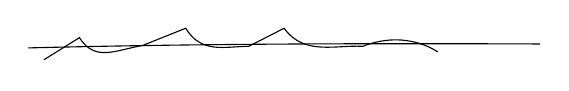
\begin{tikzpicture}[x=1cm,y=1cm]
\draw (0,0) .. controls (2,.05) and (4,.06) .. (6.5,.05);
\draw (.2,-.15) -- (.65,.13) .. controls (.85,-.18) and (1.1,-.03) .. (1.45,.03)
 -- (2,.25) .. controls (2.2,-.08) and (2.5,.02) .. (2.8,.02)
 -- (3.25,.25) .. controls (3.5,-.1) and (3.9,.04) .. (4.25,.02)
 .. controls (4.65,.18) and (5,.08) .. (5.2,-.05);
\end{tikzpicture}}

\margin{61}
\scanpage{63}
\margin{\rotatebox{180}{62}}
\mspage{- 7 -}

$(B_q)$. \uline{Il existe un sous-groupe invariant} $C$ \uline{de} $G$
\uline{qui est cyclique d'ordre premier à} $q$, \uline{et qui est tel que}
$G/C$ \uline{soit un} $q$-\uline{groupe}.

Le résultat suivant est dû à Brauer [3] et Witt [18]:

PROPOSITION 2. \uline{Soit} $G$ \uline{un groupe fini et soit} $E$
\uline{un corps de caractéristique zéro}. \uline{Supposons que, pour tout nombre premier}
$q$, \uline{et pour tout sous-groupe} $H$ \uline{de} $G$ \uline{vérifiant}
$(B_q)$, \uline{l'algèbre} $E[H]$ \uline{soit décomposée}. \uline{Alors}
$E[G]$ \uline{est décomposée}.

Rappelons brièvement la démonstration:

On commence par établir une formule:
\[
(12)\qquad 1=\underset{\lambda}{\quad}n_\lambda\varphi^*_\lambda,
\quad n_\lambda\in\underline{\underline Z},
\]
où les $\varphi_\lambda$ sont des caractères de représentations rationnelles sur
$E$ de sous-groupes $H_\lambda$ vérifiant $(B_{q_\lambda})$, et où
$\varphi^*_\lambda$ désigne le caractère de $G$ \uline{induit} par
$\varphi_\lambda$; voir Witt [18], Satz 6, ou bien Swan [14], th.4.1.

Si maintenant $\chi$ est un caractère de $G$ à valeurs dans $E$, on multiplie
(12) par $\chi$, et l'on obtient:
\[
(13)\qquad \chi=\sum n_\lambda\varphi^*_\lambda\chi
=\sum n_\lambda(\varphi_\lambda\chi)^*.
\]
Comme $\varphi_\lambda\chi$ est un caractère de $H$ à valeurs dans $E$,
l'hypothèse faite sur les $H_\lambda$ montre que c'est le caractère d'une
représentation de $H_\lambda$ rationnelle sur $E$; donc
$(\varphi_\lambda\chi)^*$ est le caractère d'une représentation de $G$
rationnelle sur $E$. La formule (13), jointe au critère (b) ci-dessus, montre
que $\chi$ est le caractère d'une représentation de $G$ rationnelle sur $E$.
Ceci ayant lieu pour tout $\chi$, la prop.1 montre que $E[G]$ est décomposée, cqfd.

3. \uline{Démonstration du théorème 3}.

Compte tenu de la prop.1, il s'agit de prouver que, \uline{si} $G$ \uline{vérifie}
$(R_p)$ \uline{et si} $\ell\ne p$, \uline{l'algèbre} $Q_\ell[G]$
\uline{est décomposée}. De plus, la prop.2 permet de supposer qu'il existe un
nombre premier $q$ tel que $G$ vérifie $(B_q)$. Nous
\scanpage{65}

\diagram{\begin{tikzcd}
\underline O_{\hat C}(\unsure{U|1})\arrow[r,rightsquigarrow]&
\underline O_{\hat C_X}(\unsure{U|1})
\end{tikzcd}}
\[
\hat C=\operatorname{Spec}S[z]\qquad
\left\{\begin{gathered}\text{induit }0\\\text{sur }C\text{ et}\\\text{sur }C'\end{gathered}\right.
\]
\[
O_{\hat C}(1)
\]

\diagram{\begin{tikzcd}
\operatorname{Pic}(\hat C)\arrow[r]&{}
\end{tikzcd}}

\margin{\deleted{\unsure{Pic $C$}}}

\diagram{\begin{tikzcd}[column sep=large,row sep=large]
\operatorname{Pic}(X)
\arrow[r,"{\text{injectif,}}","{\substack{[\text{bijectif}\\\text{dans le cas}\\X\ \unsure{\text{loc.}}\ \text{factoriel}]}}"']
\arrow[rr,bend left=30,"{\text{noyau }\unsure{\subset\underline{Z\xi}|\text{engendré}}}"]&
\operatorname{Pic}(\hat C')\arrow[r]
\arrow[dr]&
\operatorname{Pic}(C')\arrow[r,"{\text{injectif}}"',"{\substack{[\text{surjectif}\\\text{dans le}\\\unsure{\text{cas local}}\\\text{factoriel}]}}"]&
\operatorname{Pic}(\widetilde C')\\
&&\substack{\text{noyau}\\{}[\text{engendré par}\\\text{l'image de }O_X(1)}&
\end{tikzcd}}

\[
\operatorname{Pic}(X)/Z.\unsure{\xi|\zeta}\ \subset\
\operatorname{Pic}(\hat C')/Z\unsure{\xi|\zeta})
\]

\margin{\figure{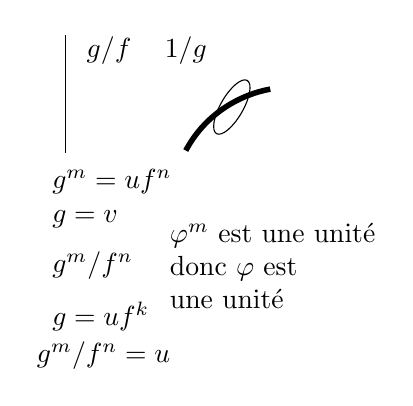
\begin{tikzpicture}[x=.65cm,y=.65cm]
\draw (-.35,3.7) -- (-.35,1.4);
\node at (.5,3.4) {$g/f$};
\node at (2,3.4) {$1/g$};
\draw[line width=2pt] (2,1.45) .. controls (2.4,2.2) and (3.1,2.55) .. (3.65,2.65);
\draw[thin,rotate around={-30:(2.9,2.3)}] (2.9,2.3) ellipse (.22 and .6);
\node[anchor=west] at (-.8,.85) {$g^m=uf^n$};
\node[anchor=west] at (-.8,.1) {$\deleted{g=\unsure{v}}$};
\node[anchor=west] at (-.8,-.8) {$\deleted{\unsure{g^m/f^n}}$};
\node[anchor=west] at (-.8,-1.8) {$g=uf^k$};
\node[anchor=west] at (-1.1,-2.55) {$\unsure{g^m/f^n=u}$};
\node[align=left,anchor=west] at (1.5,-.8)
 {$\varphi^m$ est une unité\\donc $\varphi$ est\\une unité};
\end{tikzpicture}}}

\figure{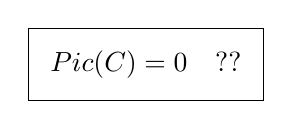
\begin{tikzpicture}
\node[draw,rectangle,inner sep=8pt] {$\operatorname{Pic}(C)=0\quad??$};
\end{tikzpicture}}

\diagram{\begin{tikzcd}[column sep=large,row sep=large]
&&0\arrow[d]&\\
&Z.\unsure{\xi|\zeta}\arrow[r,phantom,"{\unsure{=|\Rightarrow}}" description]\arrow[d]&Z\unsure{\xi|\zeta}
\arrow[d,"{\text{\textcircled{?}}}"]&\\
\unsure{0|\bullet}\arrow[r,dash]&\operatorname{Pic}(X)
\arrow[r,"{\substack{\text{injectif}\\{}[\text{surjectif}]}}"']&
\operatorname{Pic}(\hat C')
\arrow[d,"{\substack{\deleted{\text{injectif}}\\{}[\text{surjectif}]}}"]&
\unsure{\mathbin{-}}\arrow[l]\\
&\operatorname{Pic}(C)\arrow[r]&\operatorname{Pic}(C')\arrow[r]&
\operatorname{Pic}(\widetilde C')
\end{tikzcd}}

\margin{$\unsure{1|\downarrow}$}

\margin{\figure{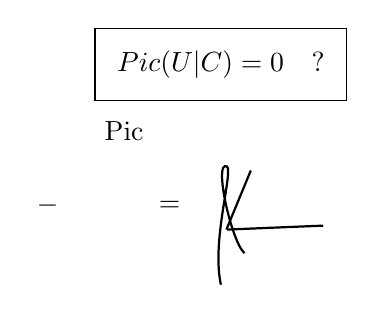
\begin{tikzpicture}
\node[draw,rectangle,inner sep=8pt] at (0,1.7) {$\operatorname{Pic}(\unsure{U|C})=0\quad?$};
\node[anchor=west] at (-1.6,.85) {Pic};
\node at (-2.2,-.1) {$-$};
\node at (-.65,-.1) {$=$};
\draw[thick] (0,-1.1) .. controls (-.12,-.55) and (.15,.3) .. (.08,.4)
 .. controls (-.1,.5) and (.13,-.55) .. (.3,-.7);
\draw[thick] (.07,-.4) -- (.38,.35);
\draw[thick] (.08,-.4) -- (1.3,-.35);
\end{tikzpicture}}}

\margin{64}
\scanpage{66}

$X-a$

\diagram{\begin{tikzcd}[column sep=tiny]
\unsure{0|\bullet}\arrow[r]&
H^0_{\unsure{a}}(X,\underline O_X^*)\arrow[r]&
H^0(X,\underline O_X^*)\arrow[r]&
H^0(U,\underline O_X^*)\arrow[r]&
H^{\unsure{1}}_a(X,\underline O_X^*)\arrow[r]&
\underset{\substack{\Vert\\0}}{H^1(X,\underline O_X)}\arrow[r]&
H^1(U,\underline O_X^*)\arrow[r]&
\underline{H^2_a(X,\underline O_X^*)}\arrow[r]&
\underline{H^2(X,\underline O_X^*)}
\end{tikzcd}}

\diagram{\begin{tikzcd}A^*\arrow[r]&\hat A^*\end{tikzcd}}
\margin{$\unsure{m}$}
\[
F\qquad H^0_a(F)
\]

\figure{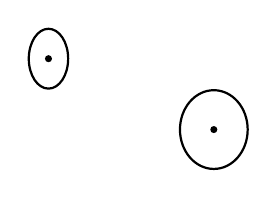
\begin{tikzpicture}[x=1cm,y=1cm]
\draw[thick] (0,1) ellipse (.25 and .38);
\fill (0,1) circle (.045);
\draw[thick] (2.1,.1) ellipse (.43 and .5);
\fill (2.1,.1) circle (.045);
\end{tikzpicture}}

\diagram{\begin{tikzcd}[column sep=large,row sep=large]
\text{loc. factoriel}\arrow[r,Rightarrow]\arrow[dr,Rightarrow]&
\inserted{\text{loc.}}\ \text{quasi-factoriel}\arrow[r,Rightarrow]&
\text{parafactoriel}\\
&\text{\unsure{1} factoriel,}\arrow[d,Rightarrow]&\\
&\text{0-factoriel,}&
\end{tikzcd}}

\diagram{\begin{tikzcd}\widetilde A\arrow[r]&\widetilde A_0\end{tikzcd}}
\deleted{$\unsure{\widetilde A_\xi}$}
\margin{$\longleftarrow$}

\[
H^1(X,\underline O_X)=0
\]

\figure{\begin{tikzpicture}[x=1cm,y=1cm]
\node at (0,.9) {$L$};
\node at (1.1,.9) {$L_B$};
\draw (2.65,1.55) -- (3.7,-.2);
\draw (3.4,1.7) .. controls (3.15,.7) and (2.95,-.35) .. (2.8,-.4);
\fill (3.13,.8) circle (.045);
\node at (5.2,1.8) {$\widetilde X$};
\node at (5.2,.8) {$X$};
\node at (9.7,2.1) {$\Rightarrow$};
\end{tikzpicture}}

\[
J\subset A\subset B
\]
\figure{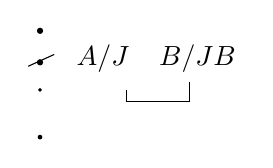
\begin{tikzpicture}[x=1cm,y=1cm]
\fill (-.6,.55) circle (.04);
\fill (-.6,.15) circle (.04);
\draw (-.75,.1) -- (-.42,.25);
\fill (-.6,-.2) circle (.025);
\fill (-.6,-.8) circle (.03);
\node at (.2,.2) {$A/J$};
\node at (1.4,.2) {$B/JB$};
\draw (.5,-.2) -- (.5,-.35) -- (1.3,-.35) -- (1.3,-.1);
\end{tikzpicture}}

\margin{\deleted{$\unsure{1-h=}$}
\[
1-h^1\unsure{=|:}2-h'-h''
\]}

\[
1-g=\sum(1-g_i)-\sum n_s\ \unsure{\ne|=}0
\]
\[
1-g=\nu-\sum g_i-\sum n_s
\]

\figure{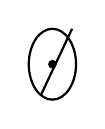
\begin{tikzpicture}[x=1cm,y=1cm]
\draw[thick] (0,0) ellipse (.3 and .45);
\draw[thick] (-.15,-.4) -- (.25,.45);
\fill (0,0) circle (.055);
\end{tikzpicture}}

\margin{\figure{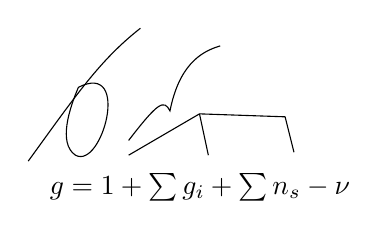
\begin{tikzpicture}[x=.75cm,y=.75cm]
\draw[thin] (0,0) .. controls (.8,1.1) and (1.2,1.7) .. (1.9,2.25);
\draw[thin] (.85,1.25) .. controls (1.75,1.7) and (1.25,-.15) .. (.8,.1)
 .. controls (.5,.3) and (.7,.9) .. (.85,1.25);
\draw (1.7,.1) -- (2.9,.8) -- (4.35,.75) -- (4.5,.15);
\draw (2.9,.8) -- (3.05,.1);
\draw (1.7,.35) .. controls (2.2,1) and (2.3,1.05) .. (2.4,.85)
 .. controls (2.55,1.6) and (2.9,1.85) .. (3.25,1.95);
\node[anchor=west] at (.2,-.45) {$g=1+\sum g_i+\sum n_s-\nu$};
\end{tikzpicture}}}

\figure{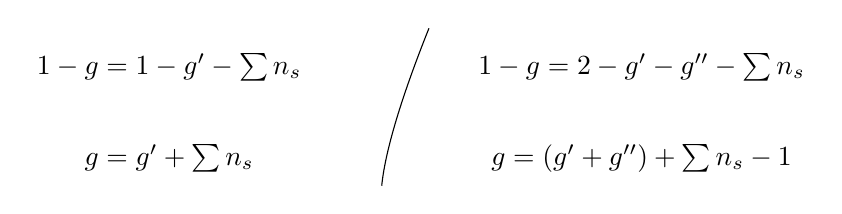
\begin{tikzpicture}[x=1cm,y=1cm]
\node at (-3,0) {$1-g=1-g'-\sum n_s$};
\node at (3,0) {$1-g=2-g'-g''-\sum n_s$};
\node at (-3,-1.15) {$g=g'+\sum n_s$};
\node at (3,-1.15) {$g=(g'+g'')+\sum n_s-1$};
\draw (.3,.5) .. controls (0,-.25) and (-.25,-1) .. (-.3,-1.5);
\end{tikzpicture}}

\figure{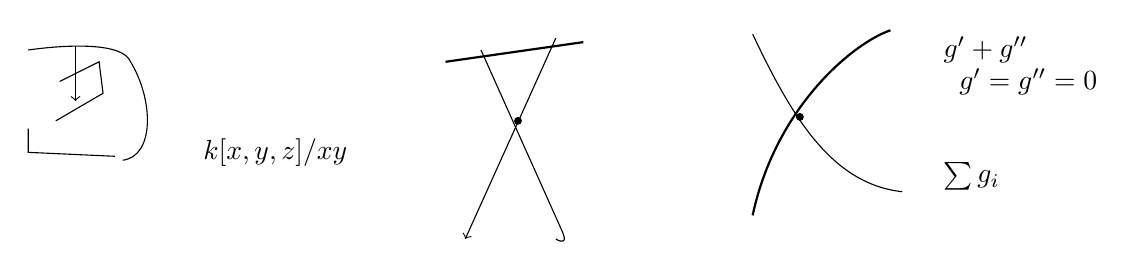
\begin{tikzpicture}[x=1cm,y=1cm]
\draw (-.5,1.05) .. controls (0,1.12) and (.7,1.15) .. (.8,.9)
 .. controls (1.1,.4) and (1.1,-.3) .. (.7,-.35);
\draw (-.5,.05) -- (-.5,-.25) -- (.6,-.3);
\draw (-.15,.15) -- (.45,.5) -- (.4,.9) -- (-.1,.65);
\draw[->] (.1,1.1) -- (.1,.4);
\node[anchor=west] at (1.6,-.25) {$k[\unsure{x},y,z]/xy$};
\begin{scope}[shift={(5.2,.1)}]
\draw[->] (1,1.1) -- (-.15,-1.45);
\draw (.05,.95) -- (1.08,-1.35) .. controls (1.15,-1.5) and (1.08,-1.5) .. (1,-1.45);
\draw[thick] (-.4,.8) -- (1.35,1.05);
\fill (.52,.05) circle (.05);
\end{scope}
\begin{scope}[shift={(8.7,.05)}]
\draw[thick] (0,-1.1) .. controls (.3,.3) and (1.3,1.1) .. (1.75,1.25);
\draw (0,1.2) .. controls (.5,.15) and (1,-.7) .. (1.9,-.8);
\fill (.6,.15) circle (.05);
\node[anchor=west] at (2.3,1) {$\deleted{g'+g''}$};
\node[anchor=west] at (2.5,.6) {$g'=g''=0$};
\node[anchor=west] at (2.3,-.6) {$\sum g_i$};
\end{scope}
\end{tikzpicture}}

\margin{65}
\scanpage{67}

$X$ schéma projectif sur $k$,\qquad $\Gamma(X,\underline O_X)\simeq\unsure{k|h}$

$C$ son cône \unsure{projetant} affine, $a$ son sommet

$\hat C$ le cône projetant projectif

\margin{\diagram{\begin{tikzcd}[column sep=small,row sep=large]
X\arrow[r,dash,"i"]\arrow[d]&X'\arrow[r,"\pi"]\arrow[d,"f"]&X\\
a\arrow[r]&\hat C\arrow[r,dash]&{}
\end{tikzcd}}
\unsure{conditions} en II 8.7.5.}

\deleted{\diagram{\begin{tikzcd}
\operatorname{Pic}(X)\arrow[r,"\pi^*","\sim"']&\operatorname{Pic}(X')
\end{tikzcd}}}
[Car $X'$ est un fibré projectif sur $X$]

donc
\[
\operatorname{Pic}(X')\overset{\unsure{f^*|\pi^*}}{\overset{\sim}{\longrightarrow}}\operatorname{Pic}(X)\times Z
\]
\deleted{[$\unsure{\underline O_{X'}(1)}$]}
\inserted{$i^*:\operatorname{Pic}(X')\mathbin{-}\operatorname{Pic}(X)$ a un noyau
$\simeq Z$, engendré par $\underline O_{X'}(1)$}

\[
\operatorname{Pic}(\hat C)\longrightarrow\operatorname{Pic}(X')
\quad\text{injectif}\quad[\text{car }f_*(\underline O_{X'})=\underline O_{\hat C}]
\]
par II 8.8.6.

\unsure{Il} s'ensuit que
\figure{\begin{tikzpicture}
\node[draw,rectangle,inner sep=8pt] (b) at (0,0)
 {$\operatorname{Pic}(\hat C)\simeq Z\overset{\sim}{\longrightarrow}
 \operatorname{Ker}[\operatorname{Pic}(X')\overset{i^*}{\mathbin{-}}\operatorname{Pic}(X)]$};
\draw (-2.9,.4) -- (-2.9,-.4);
\end{tikzpicture}}

\unsure{Soit|Sur} $C_X$ la \unsure{partie|part.} de $X'$ au-dessus de $C$,
c'est un fibré \unsure{vectoriel} de rang $1$ sur $X$.
Je dis que:
\[
\operatorname{Pic}(X)\overset{\sim}{\longrightarrow}\operatorname{Pic}(C_X)\qquad(?)
\]

\margin{faudrait supposer $X$ localement factoriel??}

Car l'hom est \deleted{\unsure{évidemment}} injectif, car son composé avec
$j^*:\operatorname{Pic}(C_X)\mathbin{-}\operatorname{Pic}(X)$,
\deleted{\unsure{si $j$ est la section nulle de $C_X$, est}}
\inserted{est} l'identité. Pour la \uline{surjectivité} on note que au-dessus
d'un ouvert convenable de $X$,

\margin{66}
